\documentclass[CMPE]{KGCOEReport}
\usepackage{float}
\usepackage{adjustbox}
\graphicspath{ {./images/} }

\newcommand{\name}{Mohammed Fareed \\ Trent Wesley}
\newcommand{\exerciseNumber}{8}
\newcommand{\exerciseDescription}{Heartrate Monitor}
\newcommand{\dateDone}{November 8, 2023}
\newcommand{\dateSubmitted}{November 29, 2023}

\newcommand{\classCode}{CMPE 460}
\newcommand{\LabSectionNum}{1}
\newcommand{\LabInstructor}{Prof.\ Hussin Ketout}
\newcommand{\TAs}{Andrew Tevebaugh \\ Colin Vo}
\newcommand{\LectureSectionNum}{1}
\newcommand{\LectureInstructor}{Prof.\ Hussin Ketout}


\begin{document}
\maketitle

\section*{Abstract}

This laboratory exercise involved the design and construction of a heartbeat detection circuit. For the detection of a heartbeat, a OPB745 reflective optical sensor can be used. This device will emit light through a finger and ideally measure reflected light which varies with the pulse within the arteries of a finger. The signal output is then filtered with a low pass filter and a high pass filter to exclude frequencies outside an expected range of heart rates. The resulting signal is then amplified by an op amp to get a more useable signal. This circuit was designed, simulated using LTspice, constructed on a breadboard, and measured. C code was written with an MSP432 microcontroller which would measure pulse based on the output of the constructed circuit. This exercise also includes the design of a PCB with the same heartbeat detection circuit. This exercise was partially successful since the circuit constructed behaved as expected with an oscilloscope generated sinusoidal signal. The circuit output was accurately used by the MSP432 to detect frequency in beats per minute. The circuit constructed was unable to detect a heartbeat using the OPB745 and the PCB was not designed.

\section*{Design Methodology}

A PPG is an instrument used to measure changes in blood volume under the skin. One use of this is to measure heart rate. A circuit was designed with the intent to measure pulse within a finger using a OPB745 reflective optical sensor.

\begin{figure}[H]
    \centering
    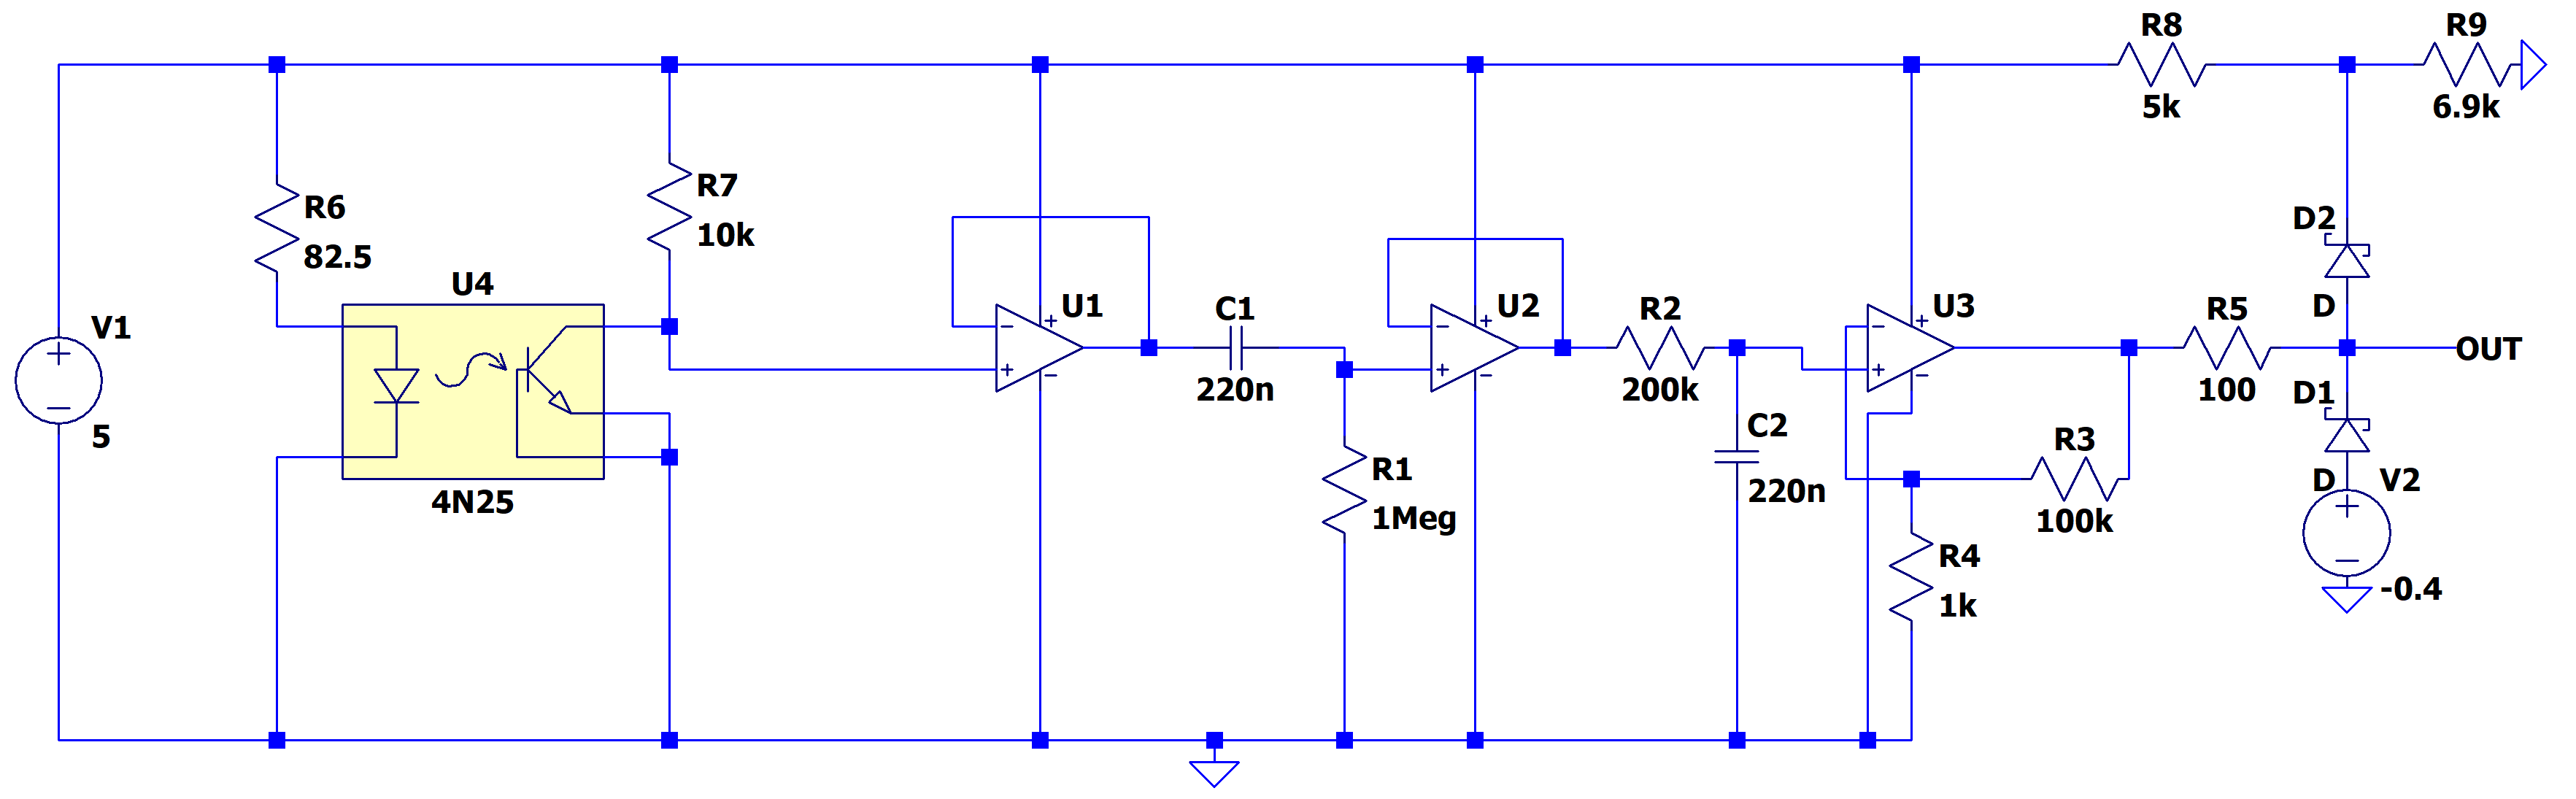
\includegraphics[width=1\textwidth]{LTspiceCompleteSchematic.png}
    \caption{LTspice Schematic}
    \label{fig:ltspiceCompleteSchematic}
\end{figure}

Figure \ref{fig:ltspiceCompleteSchematic} shows the complete schematic designed. The 4N25 represents the OPB745. A 5V source is used to provide power to the OPB745, op amps, and a Schottky diode. Voltage division occurs between the 10k$\Omega$ rseistor and the photodetector. This signal then goes to voltage follower op amp which isolates the signal from the next stage. The signal is then filtered by a passive high pass RC filter. This filter has a cut off frequency of 0.7Hz which is 40bpm. The equation to for the high pass filter design is shown below.

\begin{equation}
R = \frac{1}{2*\pi*C*\text{f}_\text{c}} = \frac{1}{2*\pi*220nF*0.7Hz} = 1M\Omega \label{eq:HighPass}
\end{equation}

With a cut off frequency of 0.7Hz and a capacitor value of 220nF, \ref{eq:HighPass} shows that the appropriate resistor value is 1M$\Omega$. The signal from the high pass filter then goes through another voltage follower for isolation between stages. Next, the signal is filtered by a passive low pass RC filter. This filter has a cut off frequency of 3.5Hz which is 210bpm.  The equation to for the low pass filter design is shown below.

\begin{equation}
R = \frac{1}{2*\pi*C*\text{f}_\text{c}} = \frac{1}{2*\pi*220nF*3.5Hz} = 200k\Omega \label{eq:LowPass}
\end{equation}

With a cut off frequency of 3.5Hz and a capacitor value of 220nF, \ref{eq:LowPass} shows that the appropriate resistor value is 200k$\Omega$. After passing through the low pass filter, the signal is amplified by an op amp. To make the signal scale up to about 3.3V, a gain of 101 was implemented. The calculation for resistor values is shown in Figure \ref{eq:amplify}.

\begin{equation}
\text{Gain} = 101 = 1 + \frac{\text{R}_\text{a}}{\text{R}_\text{b}} = 1 + \frac{100,000\Omega}{1,000\Omega} \label{eq:amplify}
\end{equation}

After amplification and filtering, the signal goes through one last stage consisting of surge protection. A 100$\Omega$ resistor was added and two Schottky diodes were placed around the output. The upper diode is attached to 2.9V from voltage division and the lower diode is attached to -0.4V. This ensures that voltages above 3.3V and below 0V will be pulled away from the output.

\section*{Results and Analysis}

The circuit was simulated using LTspice, constructed on a breadboard, and then tested and compared to the simulation results. First, the high pass filter of the circuit was simulated using the schematic shown in Figure \ref{fig:ltspiceHighPassSchematic}.

\begin{figure}[H]
    \centering
    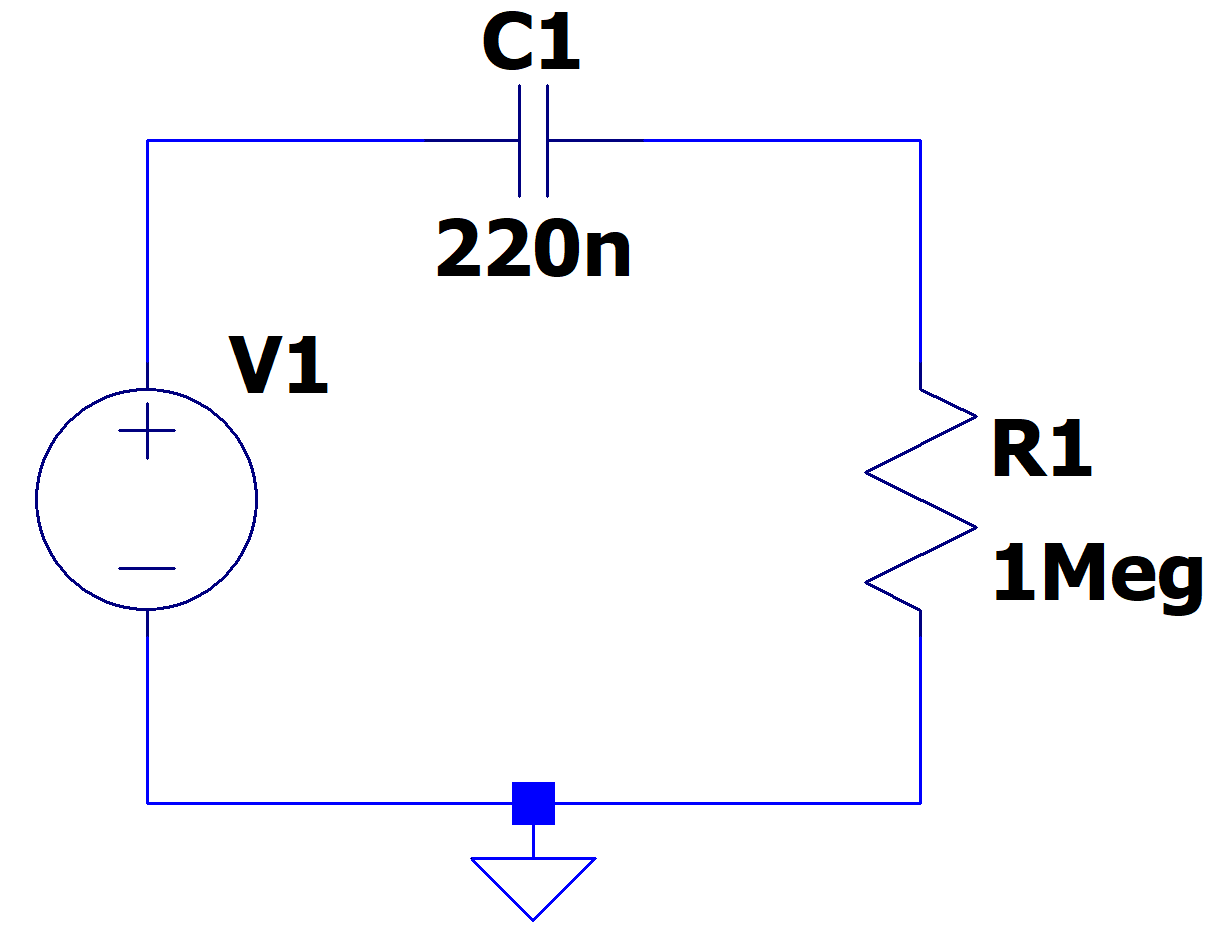
\includegraphics[width=0.35\textwidth]{HighPass.png}
    \caption{High-Pass Filter Schematic}
    \label{fig:ltspiceHighPassSchematic}
\end{figure}

The figure shows that the filter was simulated using a function generator with a 1 V, with a 220 nF capacitor and a 1 M$\Omega$ resistor. The complete circuit was then simulated using an AC sweep with a logarithmic scale from 100 mHz to 100 Hz.

Figure \ref{fig:highPassSim} shows the simulation of the high-pass filter of the circuit, performed using an AC sweep with a logarithmic scale from 100 mHz to 100 Hz.

\begin{figure}[H]
    \centering
    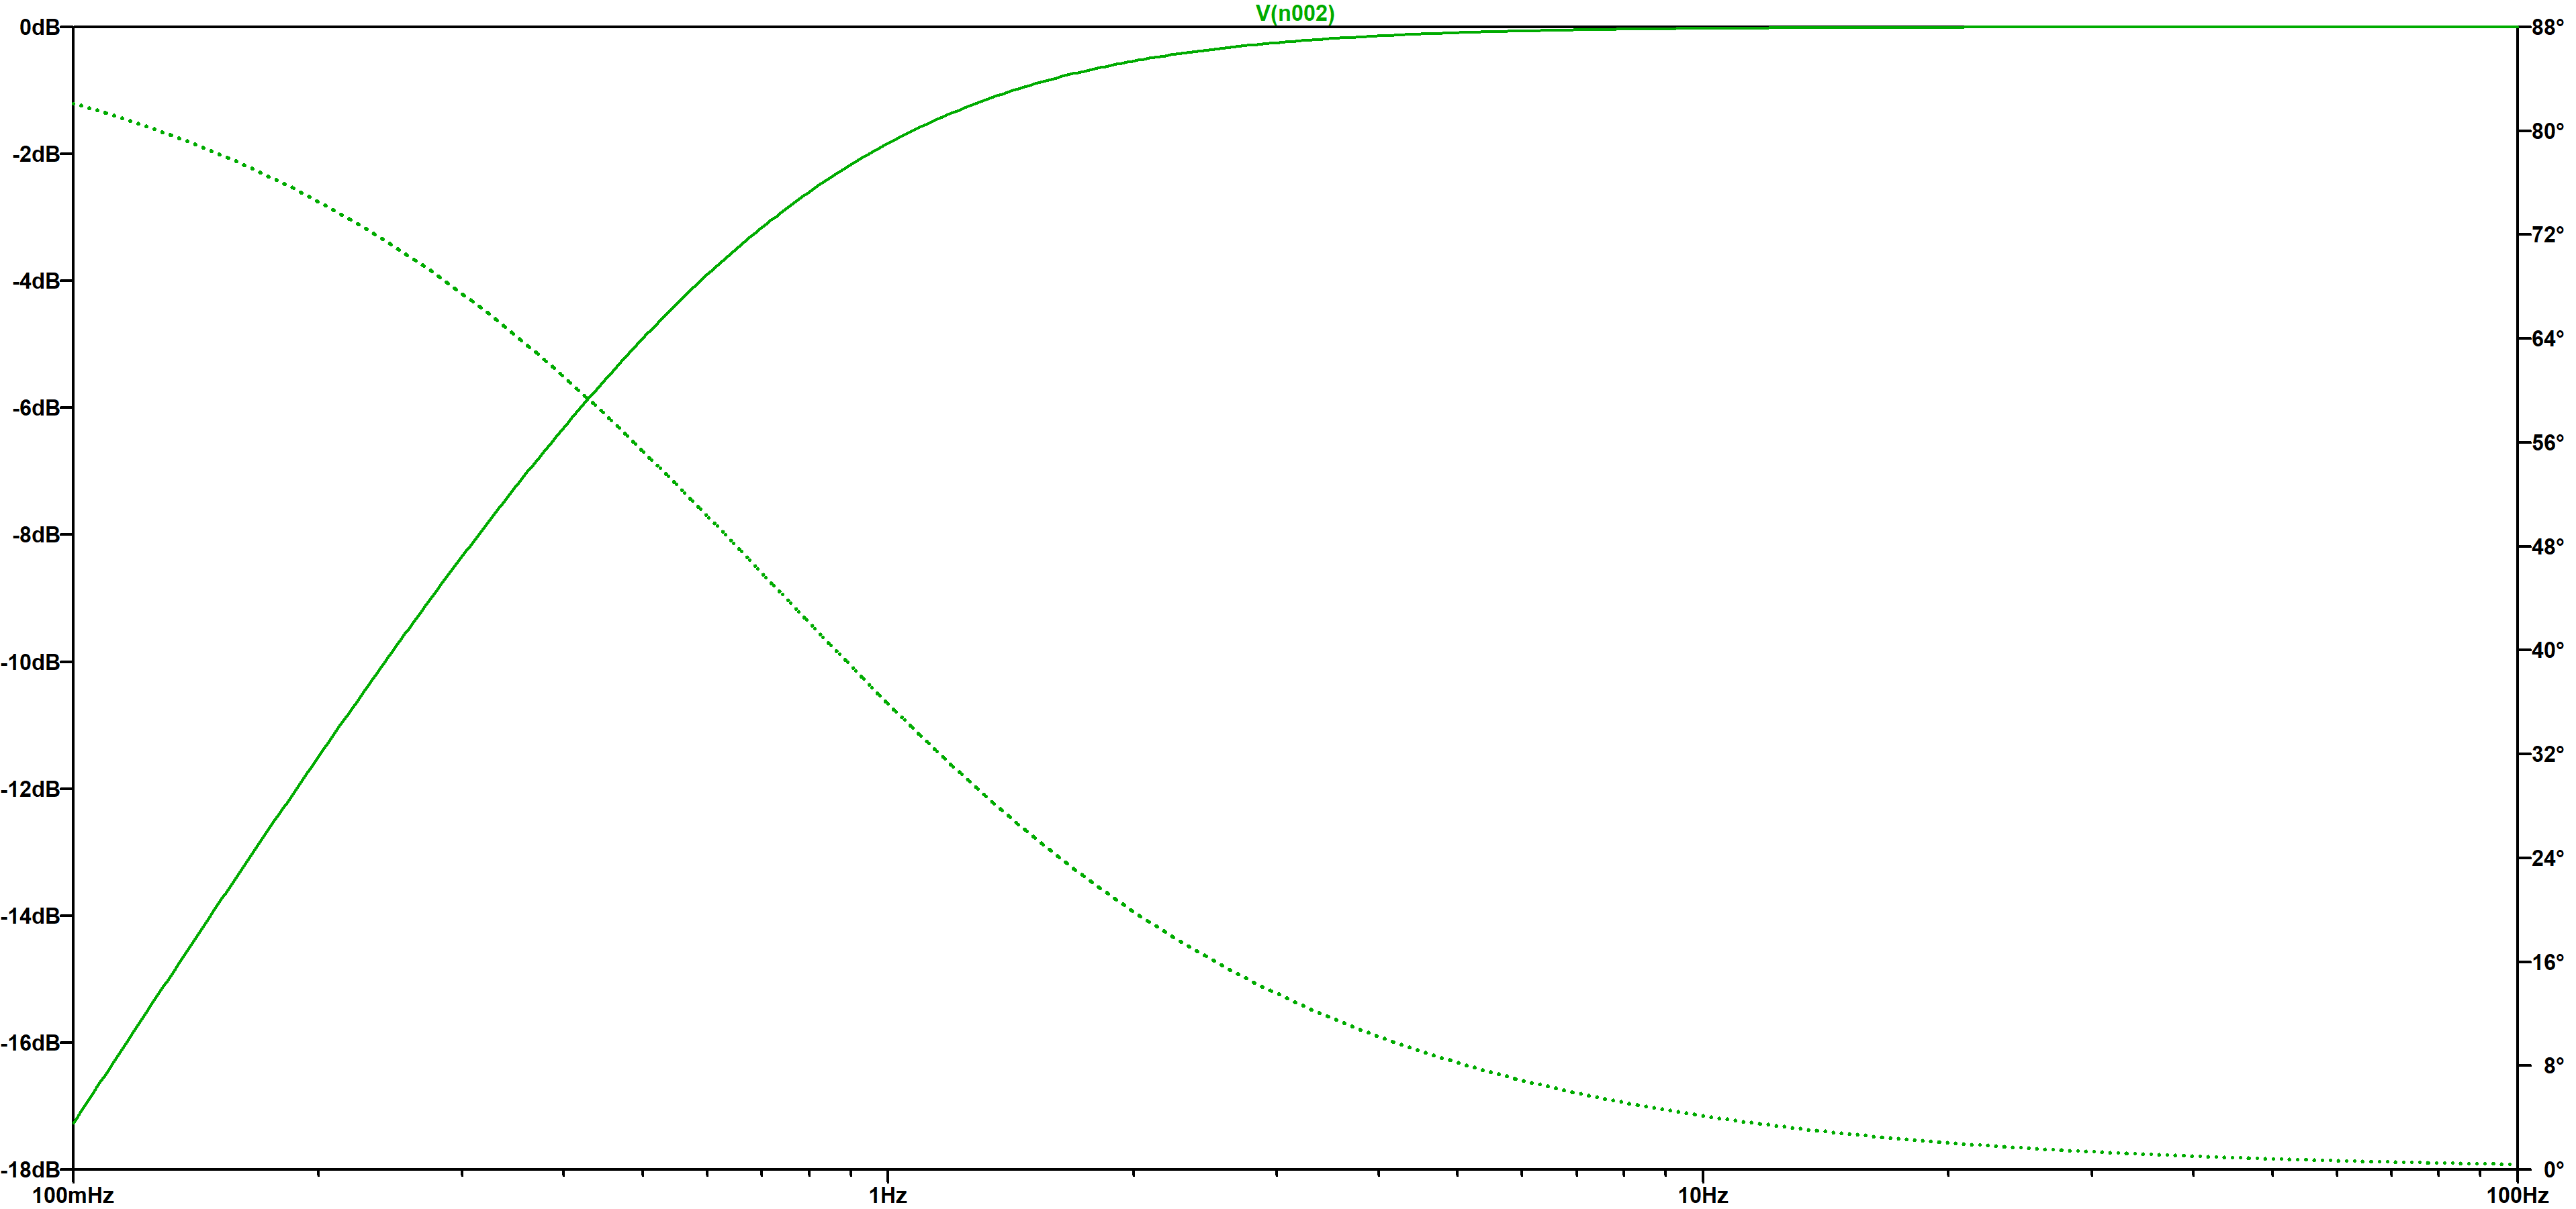
\includegraphics[width=1\textwidth]{SimFreqHighPass.png}
    \caption{High-Pass Filter Bode Simulation}
    \label{fig:highPassSim}
\end{figure}

The figure shows that the gain of the circuit is approximately 0 in the pass band, decreasing as the frequency decreases. The figure also shows that the phase shift of the circuit is approximately 90 degrees in the pass band, decreasing to 0 as the frequency decreases. The cutoff frequency of the circuit is approximately 0.7 Hz, which is equal to the calculated value.

The high-pass filter of the circuit was constructed on a breadboard and tested using an oscilloscope and a function generator at different input frequencies and the resulting voltage gain and phase shift were plotted. Figure \ref{fig:highPassBode} shows the resulting Bode plot.

\begin{figure}[H]
    \centering
    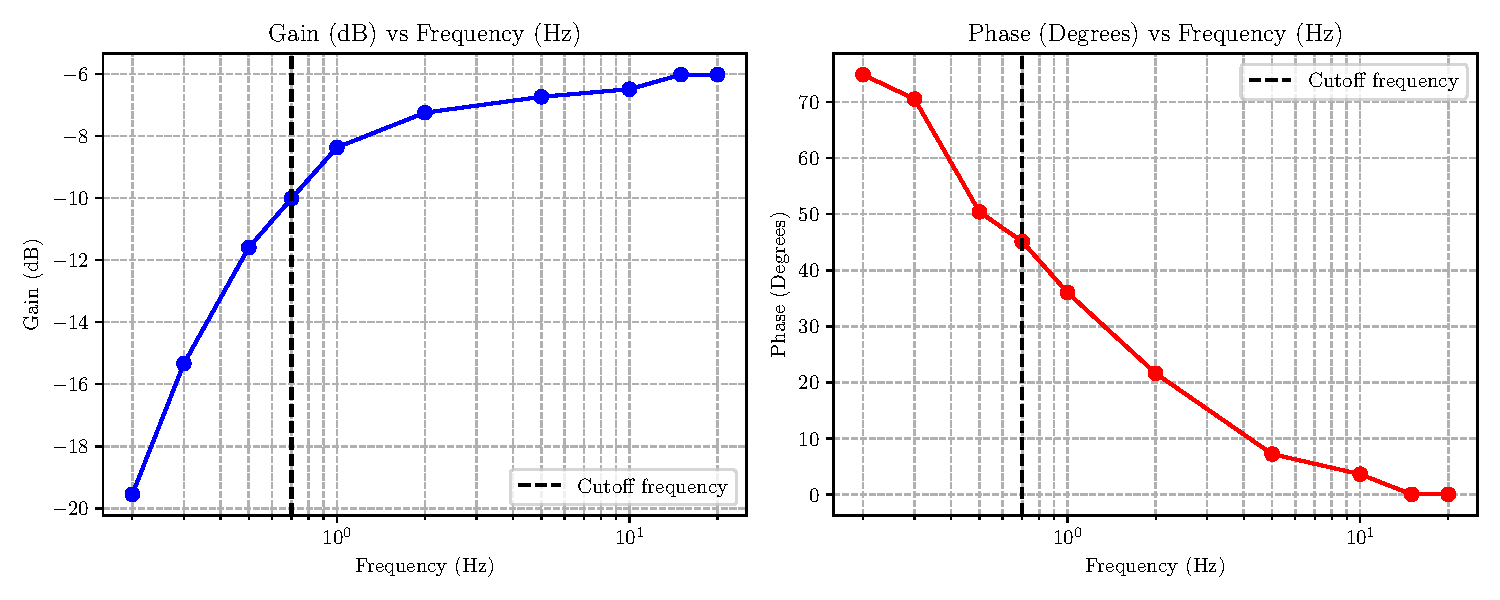
\includegraphics[width=1\textwidth]{high_pass_plot.pdf}
    \caption{High-Pass Filter Bode Plot}
    \label{fig:highPassBode}
\end{figure}

The figure shows that the calculated cutoff frequency of 0.7 Hz is approximately correct. The cutoff frequency on the plot is slightly higher than the calculated value, using -9 dB as the cutoff point (3 dB less than the maximum gain). The plot shows that the phase shift of the circuit is approximately 45 degrees at the cutoff frequency, decreasing to 0 degrees at higher frequencies. The phase shift has the general behavior of increasing from 75 to 0 degrees as the frequency increases.

The results show that the simulation and constructed circuit are similar, with the constructed circuit having a slightly higher cutoff frequency and a slightly lower phase shift at the cutoff frequency. The constructed circuit also has a lower maximum gain (-6 dB) than the simulated circuit (0 dB), which is approximately half of the simulated value. This decrease in gain propagates through the rest of the circuit.

\bigskip

The low pass filter of the circuit was simulated using the schematic shown in Figure \ref{fig:ltspiceLowPassSchematic}.

\begin{figure}[H]
    \centering
    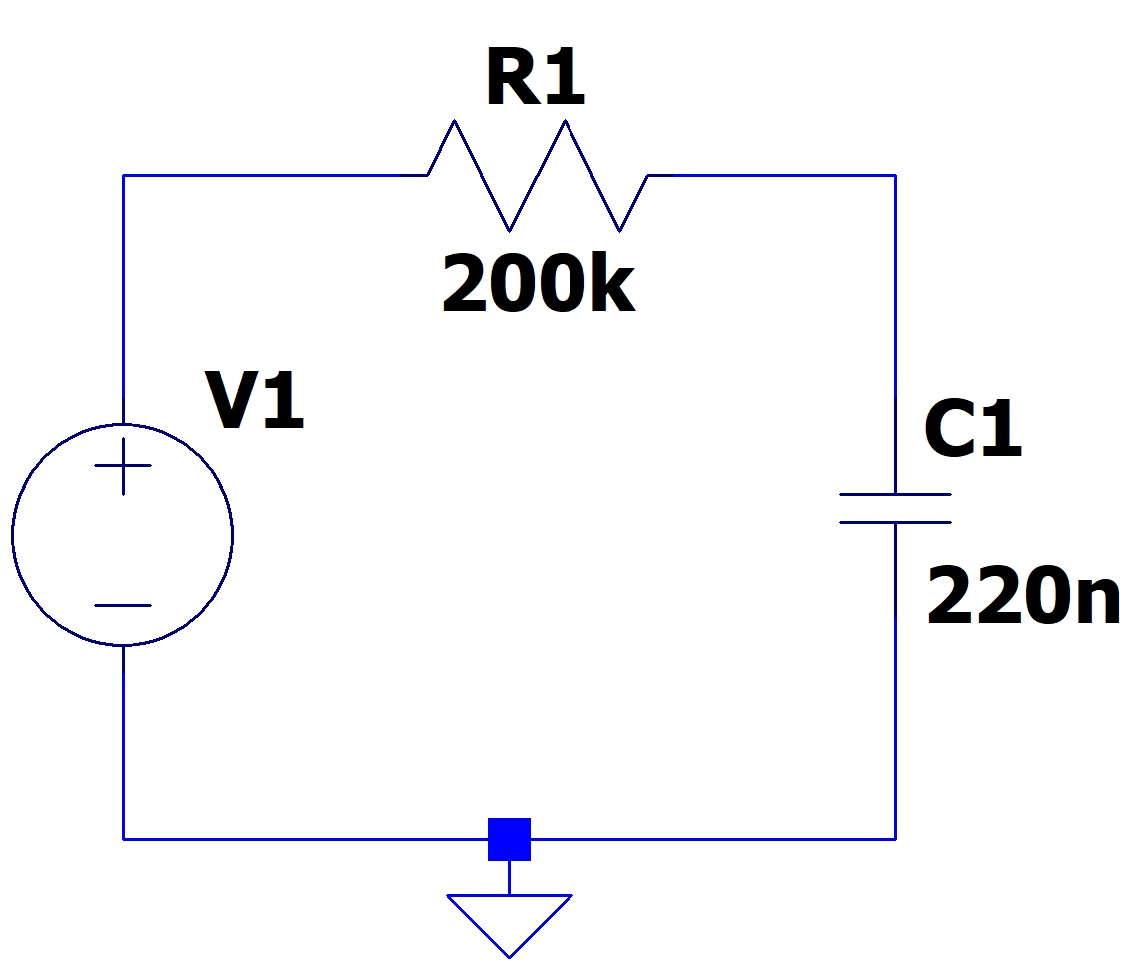
\includegraphics[width=0.35\textwidth]{LowPass.png}
    \caption{Low-Pass Filter Schematic}
    \label{fig:ltspiceLowPassSchematic}
\end{figure}

The figure shows that the filter was simulated using a function generator with a 1 V, with a 220 nF capacitor and a 200 k$\Omega$ resistor. The complete circuit was then simulated using an AC sweep with a logarithmic scale from 100 mHz to 100 Hz.

Figure \ref{fig:lowPassSim} shows the simulation of the low-pass filter of the circuit, performed using an AC sweep with a logarithmic scale from 100 mHz to 100 Hz.

\begin{figure}[H]
    \centering
    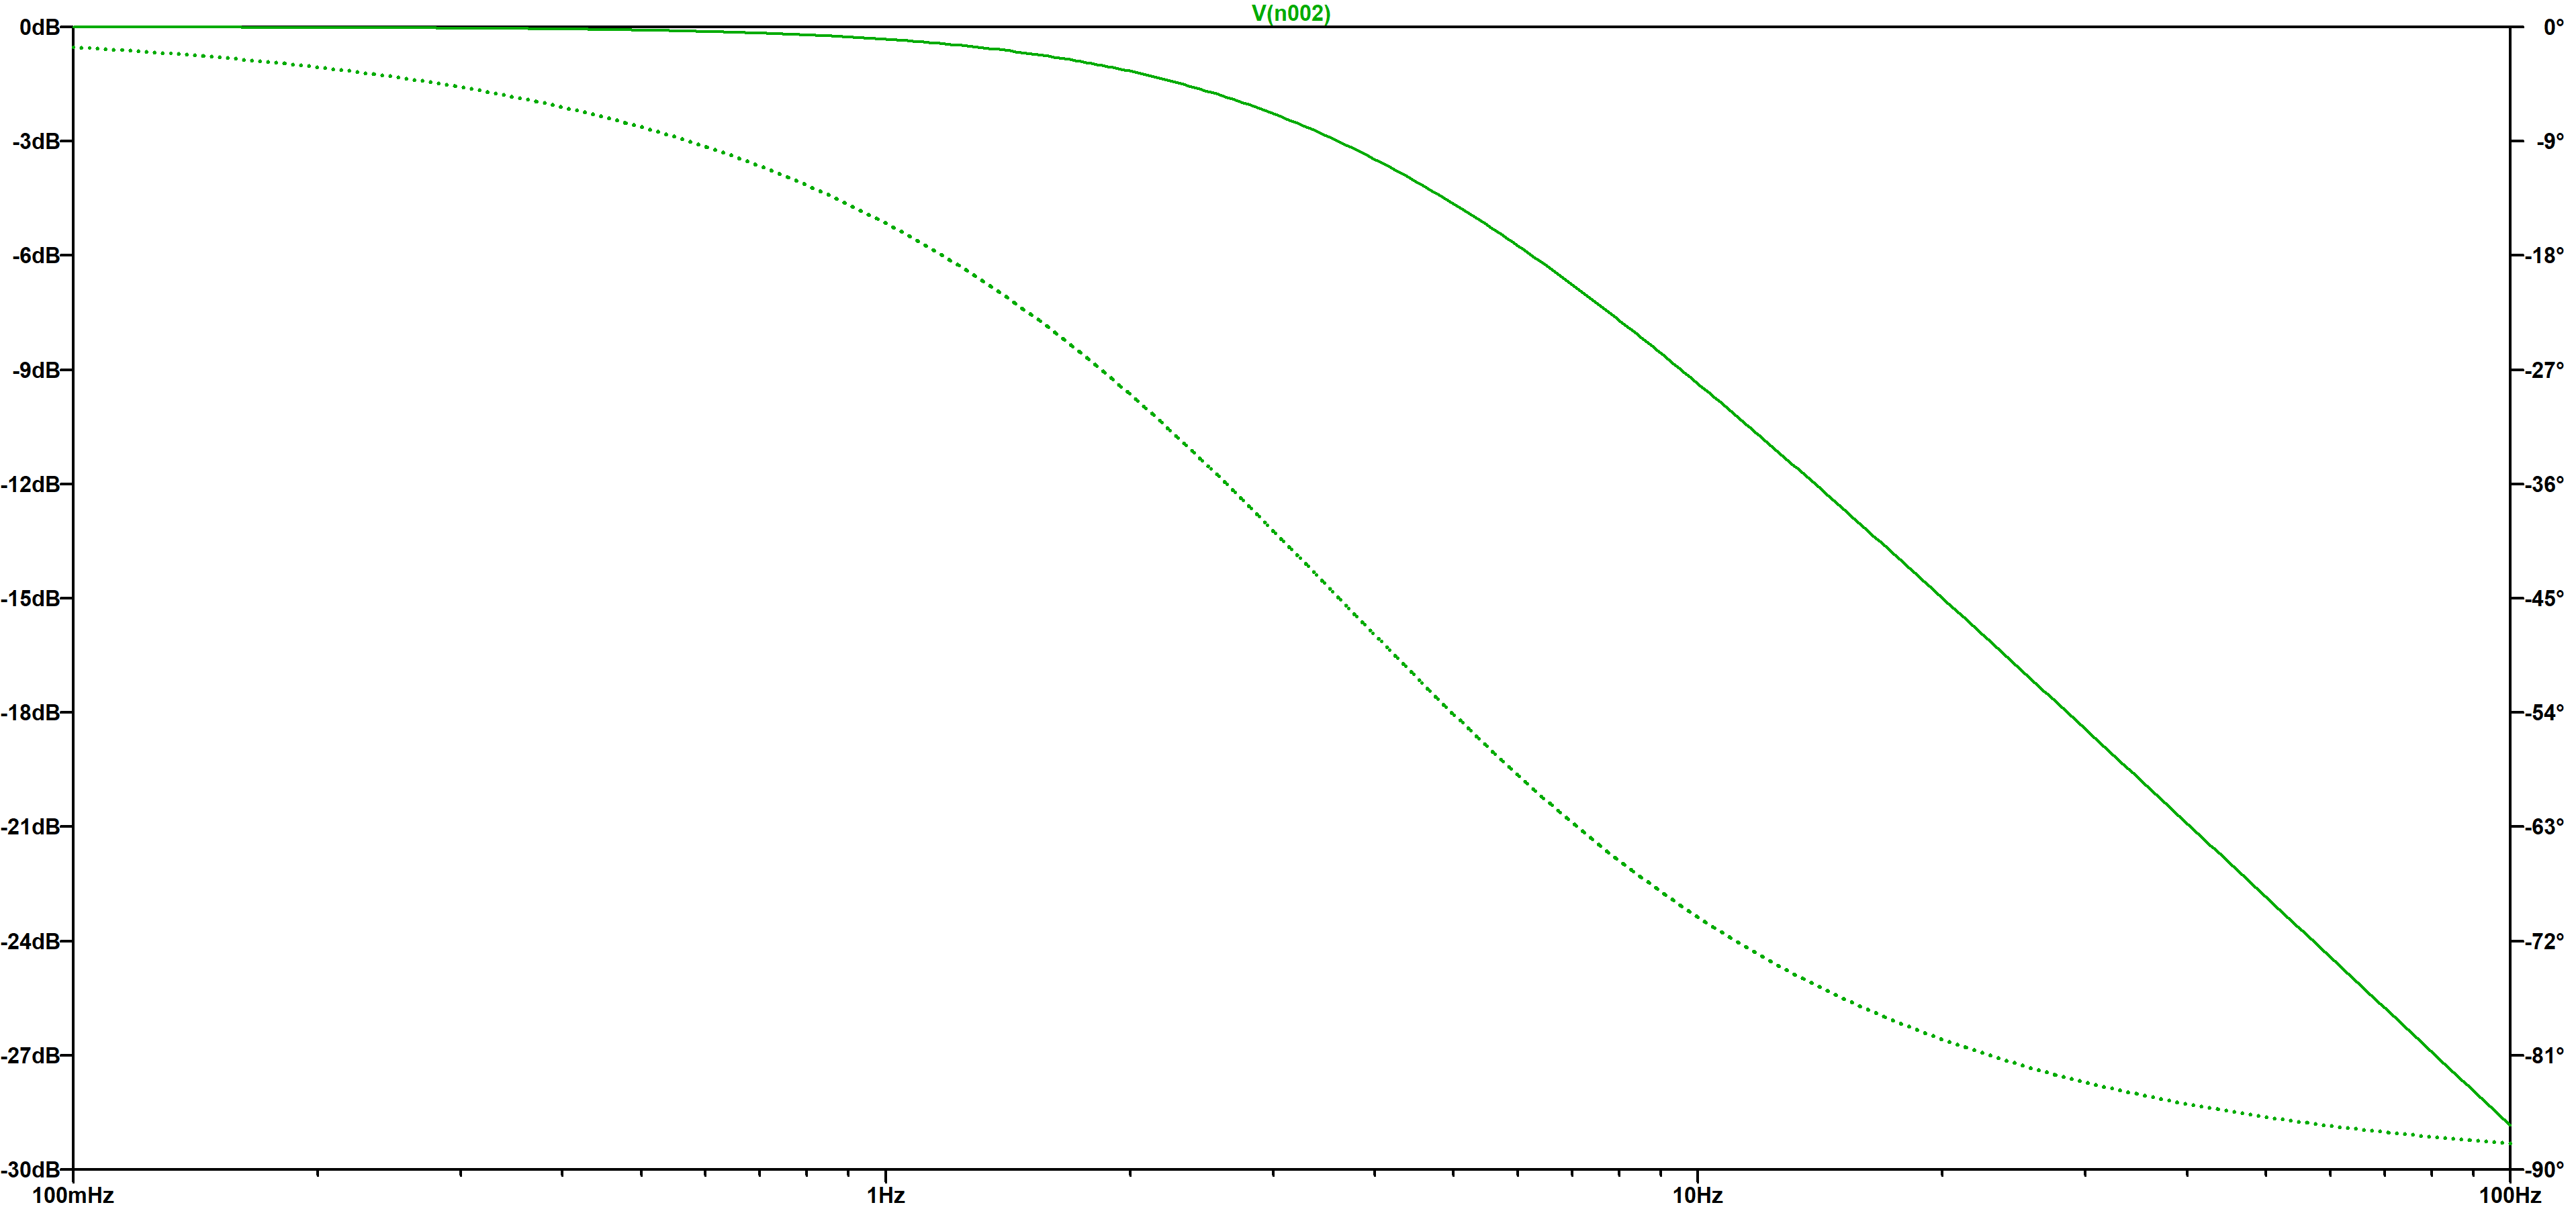
\includegraphics[width=1\textwidth]{SimFreqLowPass.png}
    \caption{Low-Pass Filter Bode Simulation}
    \label{fig:lowPassSim}
\end{figure}

The figure shows that the gain of the circuit is approximately 0 in the pass band, increasing as the frequency increases. The figure also shows that the phase shift of the circuit is approximately 0 degrees in the pass band, decreasing to -90 degrees as the frequency increases. The cutoff frequency of the circuit is approximately 3.5 Hz, which is equal to the calculated value.

The low-pass filter of the circuit was constructed on a breadboard and tested using an oscilloscope and a function generator at different input frequencies and the resulting voltage gain and phase shift were plotted. Figure \ref{fig:lowPassBode} shows the resulting Bode plot.

\begin{figure}[H]
    \centering
    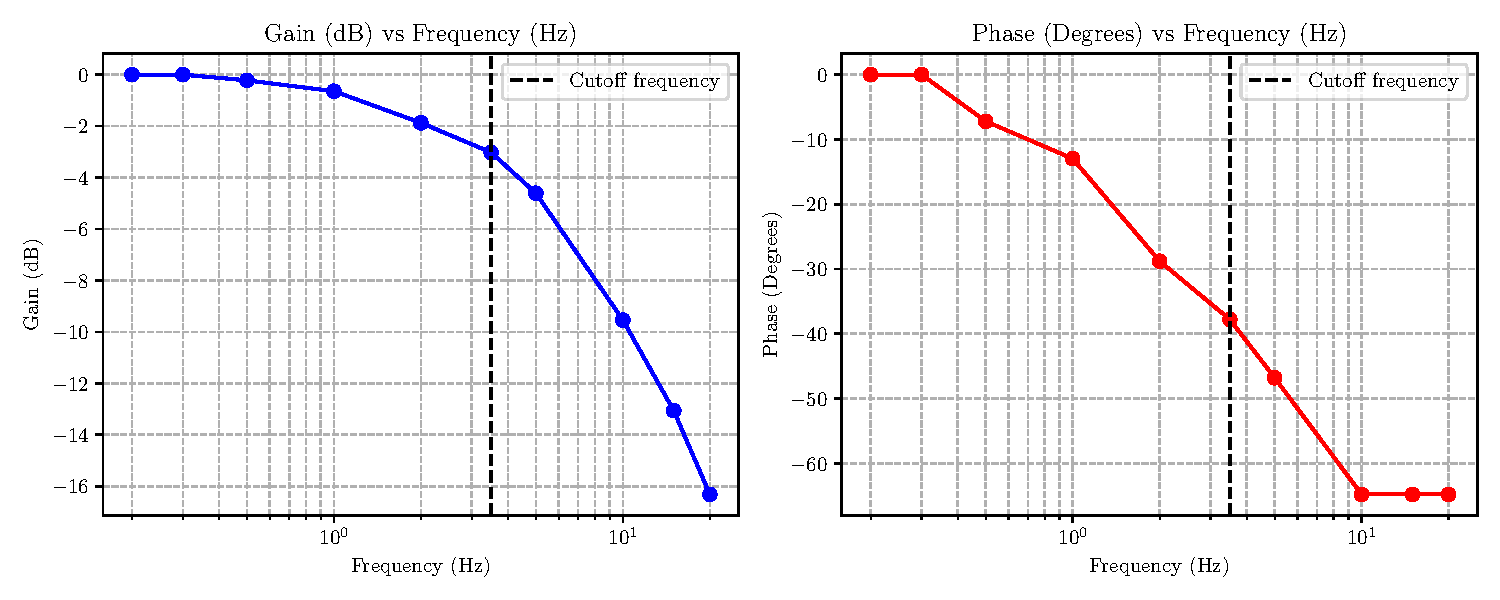
\includegraphics[width=1\textwidth]{low_pass_plot.pdf}
    \caption{Low-Pass Filter Bode Plot}
    \label{fig:lowPassBode}
\end{figure}

The figure shows that the calculated cutoff frequency of 3.5 Hz is approximately correct. The cutoff frequency on the plot falls at the calculated value, using -3 dB as the cutoff point (3 dB less than the maximum gain). The phase shift of the circuit is approximately -38 degrees at the cutoff frequency, decreasing to -65 degrees at higher frequencies, which is the expected behavior. The phase shift has the general behavior of decreasing from 0 to -65 degrees as the frequency increases.

The results show that the simulation and constructed circuit are very similar, with no significant differences between the two.

\bigskip

The band pass filter of the circuit was simulated by combining the high-pass and low-pass filters. Figure \ref{fig:bandPassSim} shows the simulation of the band-pass filter of the circuit, performed using an AC sweep with a logarithmic scale from 100 mHz to 100 Hz.

\begin{figure}[H]
    \centering
    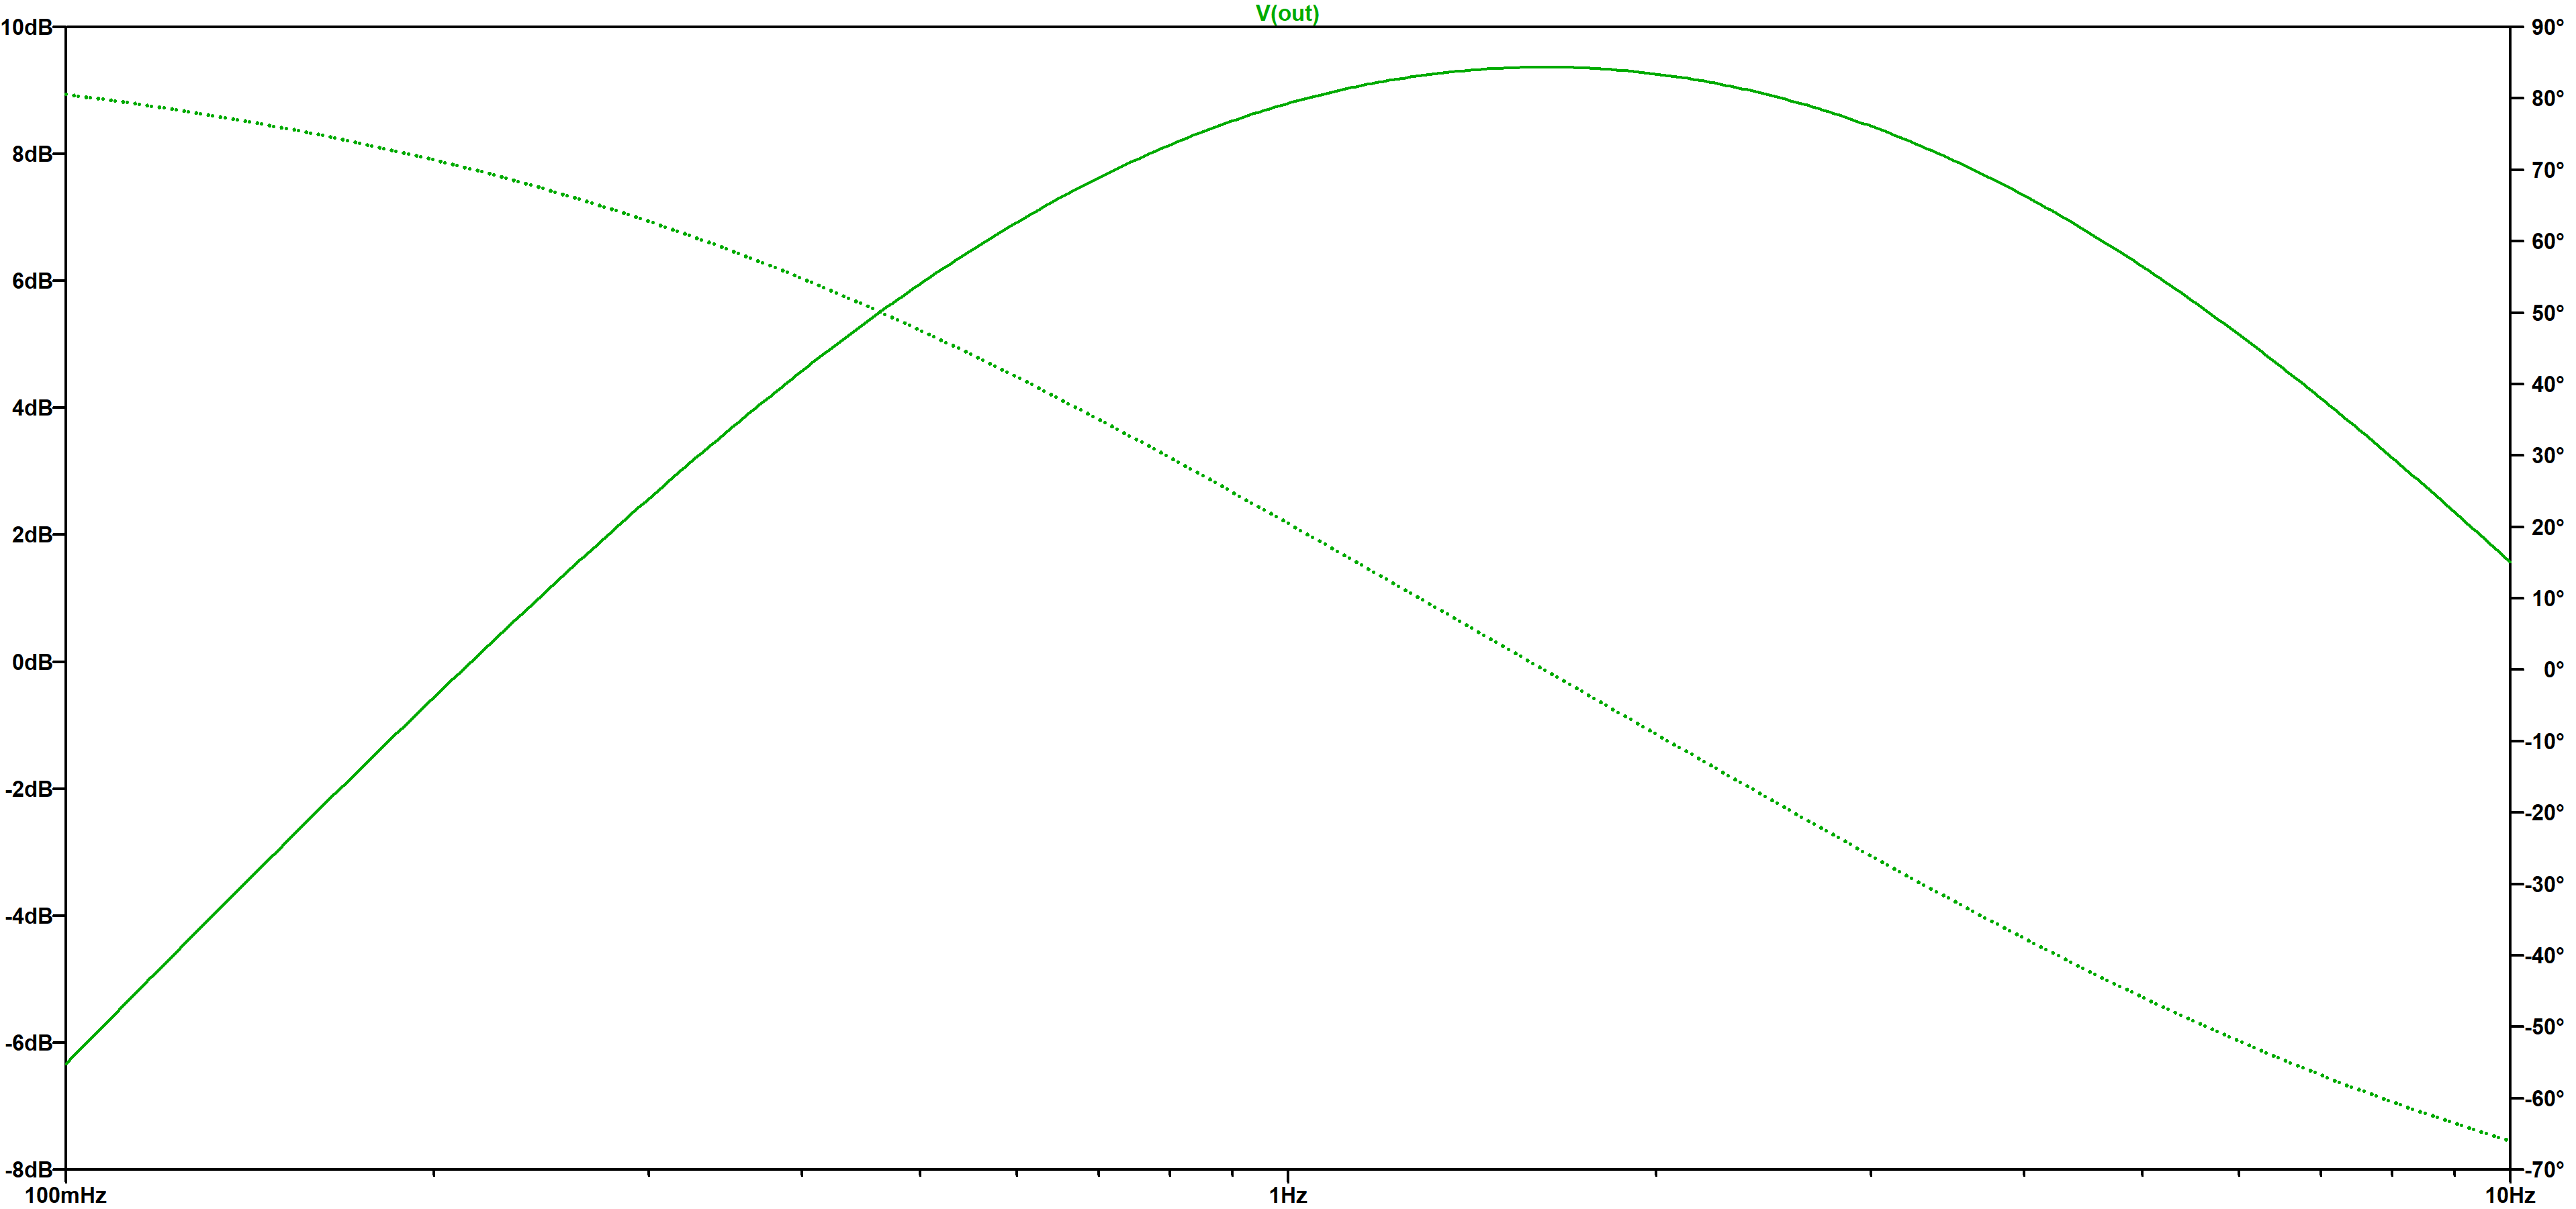
\includegraphics[width=1\textwidth]{SimFreqBandPass.png}
    \caption{Band-Pass Filter Bode Simulation}
    \label{fig:bandPassSim}
\end{figure}

The figure shows that the gain of the circuit is approximately -3 and -1 in the pass band, with cutoff frequencies of 0.7 Hz and 3.5 Hz, which matches the calculated values. The figure also shows that the phase shift of the circuit is approximately 80 degrees at low frequencies (around 100 mHz) and -80 degrees at high frequencies (around 100 Hz), which is the expected behavior. The phase shift has the general behavior of decreasing from 80 to -80 degrees as the frequency increases. The phase shift is approximately 50 degrees at the lower cutoff frequency and -25 degrees at the upper cutoff frequency, which is the expected behavior.

The band-pass filter of the circuit was constructed on a breadboard and tested using an oscilloscope and a function generator at different input frequencies and the resulting voltage gain and phase shift were plotted. Figure \ref{fig:bandPassBode} shows the resulting Bode plot.

\begin{figure}[H]
    \centering
    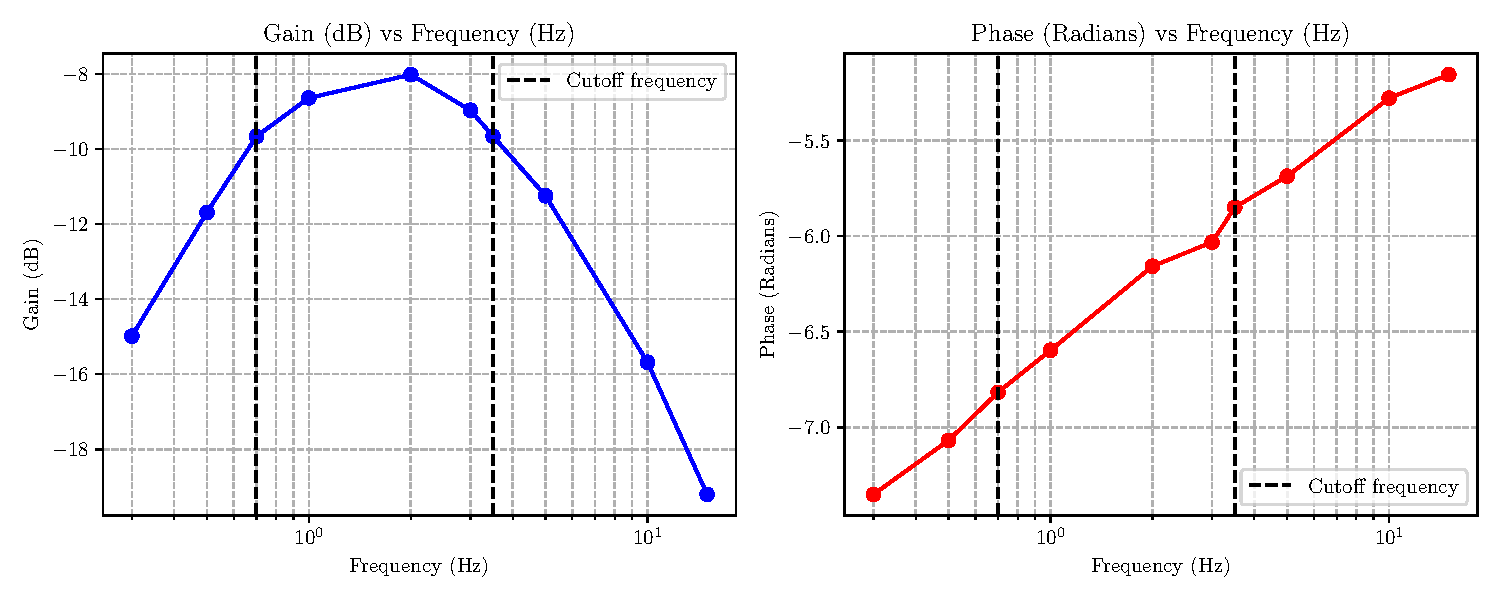
\includegraphics[width=1\textwidth]{band_pass_plot.pdf}
    \caption{Band-Pass Filter Bode Plot}
    \label{fig:bandPassBode}
\end{figure}

The figure shows that the calculated cutoff frequencies of 0.7 Hz and 3.5 Hz are approximately correct. Using -11 dB as the cutoff point (3 dB less than the maximum gain), the lower cutoff frequency is slightly lower than the calculated value and the upper cutoff frequency is slightly higher than the calculated value. The phase shift of the circuit is approximately 30 degrees at the lower cutoff frequency, decreasing to -25 degrees at the upper cutoff frequency, which is the expected behavior. The phase shift has the general behavior of decreasing from 60 to -65 degrees as the frequency increases.

The results show that the simulation and constructed circuit are similar, with the constructed circuit having a slightly lower lower cutoff frequency and a slightly higher upper cutoff frequency. The constructed circuit also has a lower maximum gain (-8 dB) than the simulated circuit (-2 dB), which is attributed to the decreased gain of the high-pass filter of the circuit. The phase shift of the constructed circuit is also slightly lower than the simulated circuit at the lower cutoff frequency.

\bigskip

The PPG circuit was then constructed and simulated in LTspice. Figure \ref{fig:ltspiceSchematic} shows the schematic of the complete circuit constructed in LTspice.

\begin{figure}[H]
    \centering
    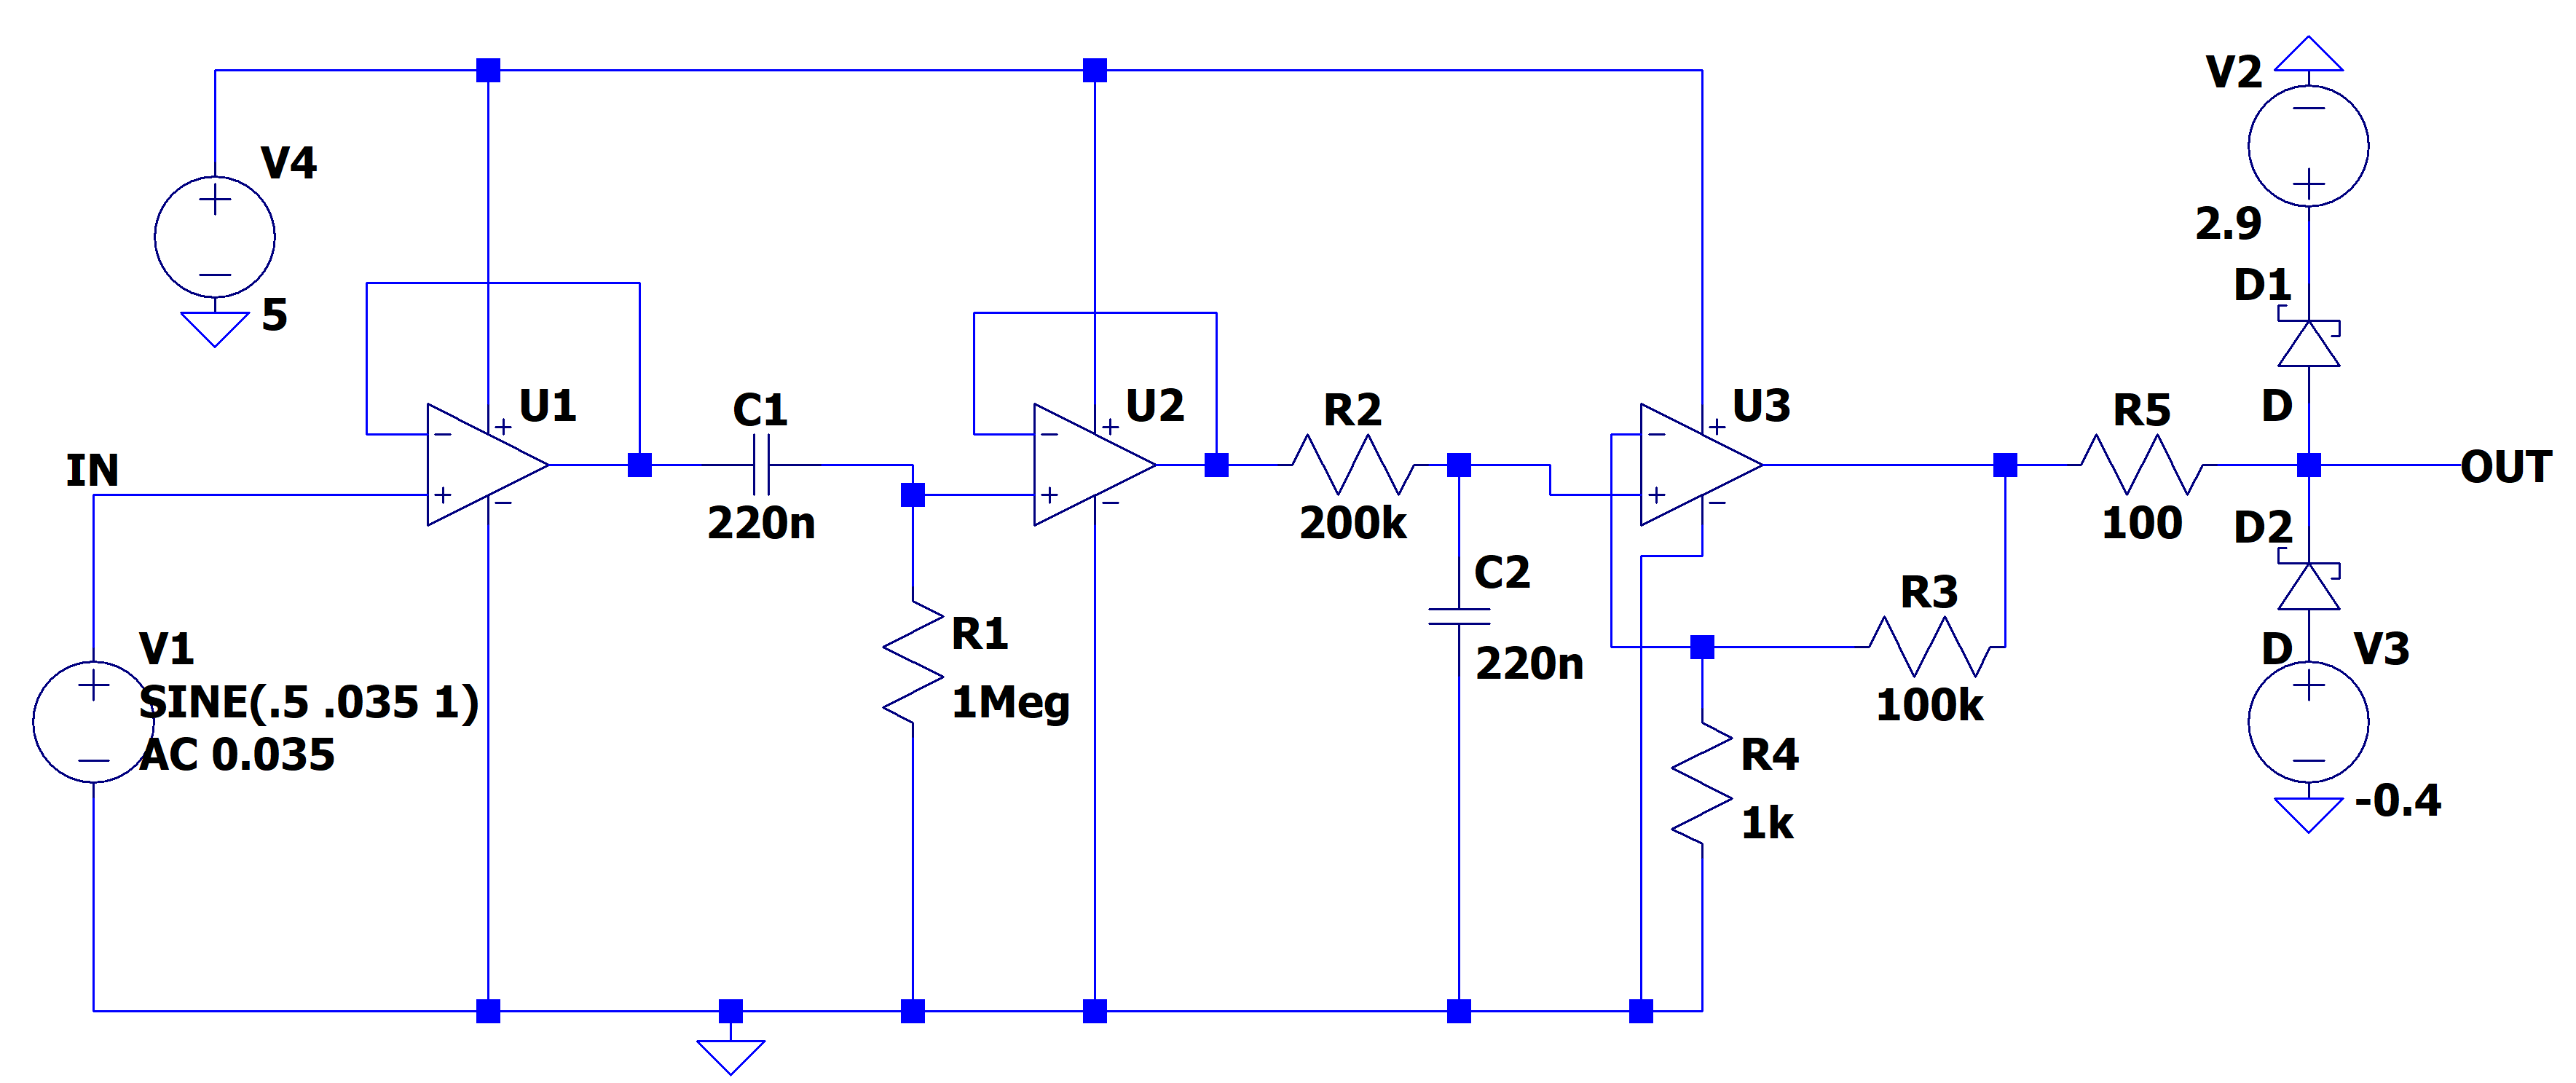
\includegraphics[width=1\textwidth]{LTspiceSchematic.png}
    \caption{LTspice Schematic}
    \label{fig:ltspiceSchematic}
\end{figure}

The figure shows that the OPB745 is simulated using a function generator with a 1 V amplitude and a frequency of 1 Hz, and the circuit is constructed using the appropriate components. The complete circuit was then simulated using an AC sweep with a logarithmic scale from 100 mHz to 100 Hz. Figure \ref{fig:completeSim} shows the simulation of the complete circuit.

\begin{figure}[H]
    \centering
    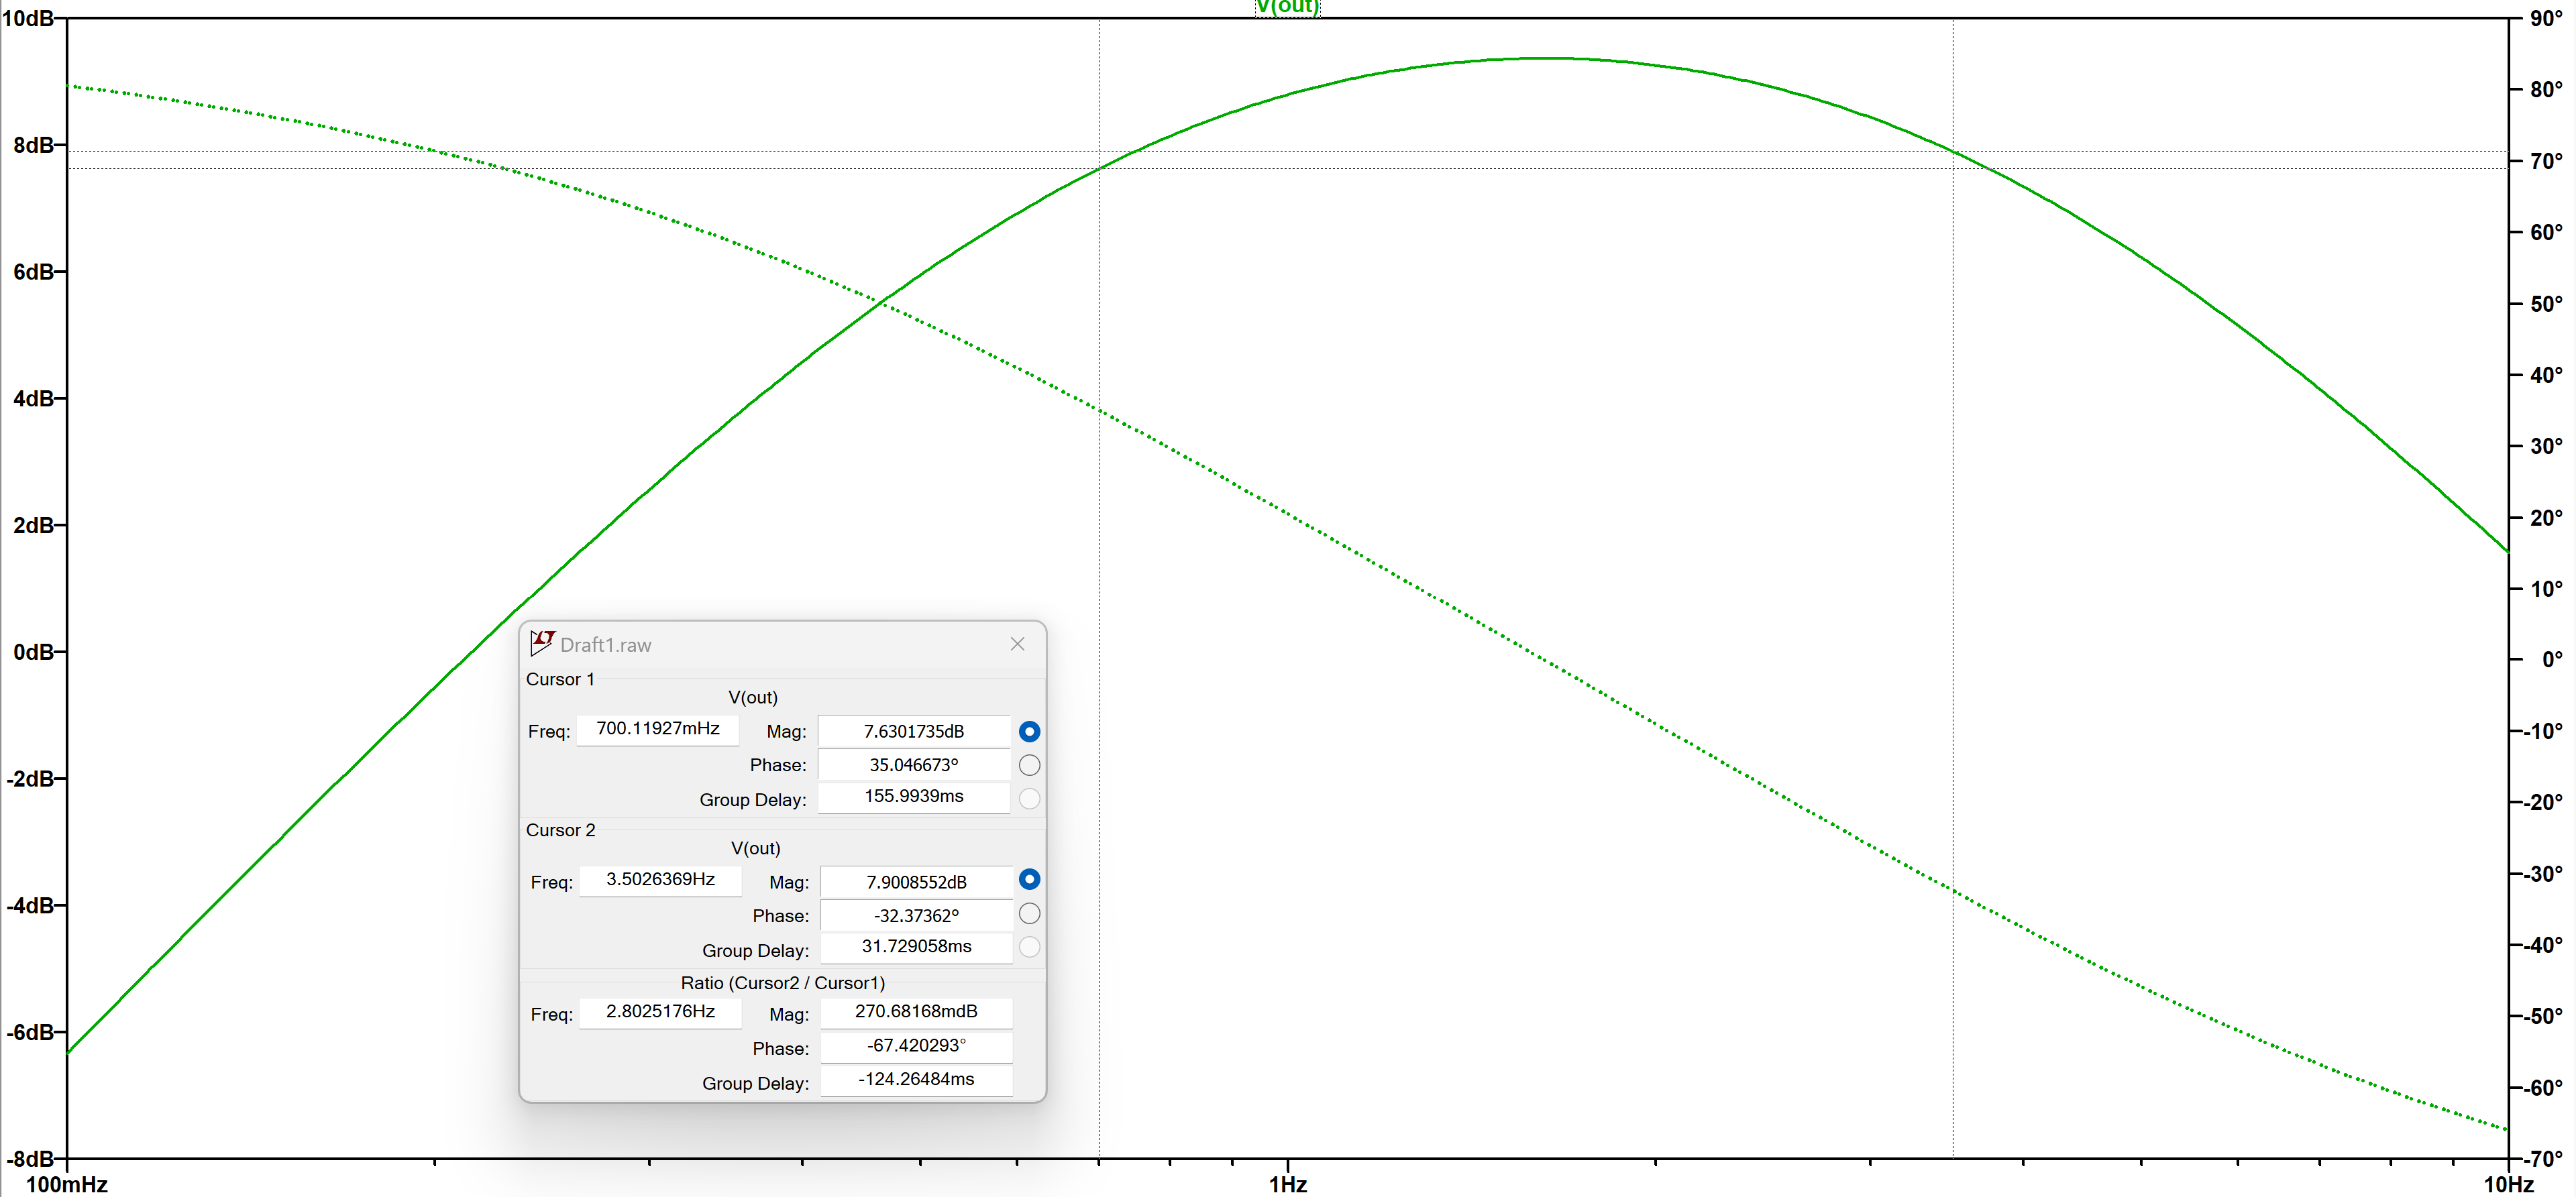
\includegraphics[width=1\textwidth]{SimFreqOutputValues.png}
    \caption{Complete Circuit Bode Simulation}
    \label{fig:completeSim}
\end{figure}

The figure shows that the gain of the complete circuit has a maximum of around 9.5 dB at 1.5 Hz. The calculated cutoff frequencies of 0.7 Hz and 3.5 Hz are at 7.6 dB and 7.9 dB, respectively, which is approximately correct. The figure also shows that the phase shift of the circuit is approximately 80 degrees at low frequencies (around 100 mHz) and -65 degrees at high frequencies (around 100 Hz), which is close to the expected values. The phase shift has the general behavior of decreasing from 80 to -65 degrees as the frequency increases. The phase shift is approximately 30 degrees at the lower cutoff frequency and -30 degrees at the upper cutoff frequency, which is also close to the expected values.

The final output of the circuit was then simulated using a time domain simulation with an input of a 1 V sinusoidal wave with a frequency of 1 Hz. Figure \ref{fig:timeSim} shows the simulation of the complete circuit.

\begin{figure}[H]
    \centering
    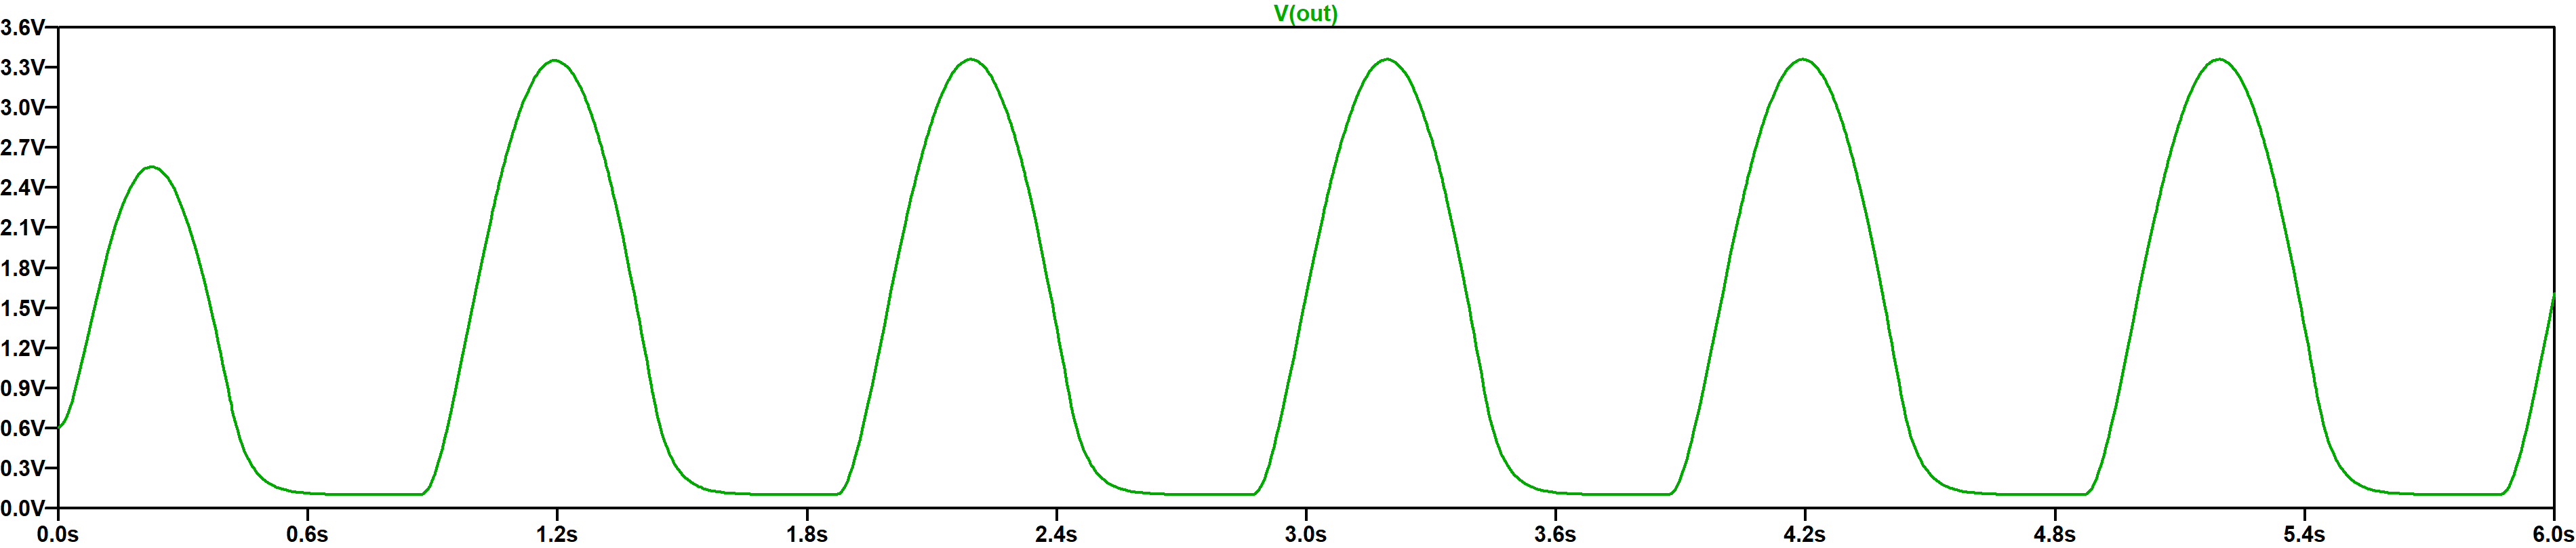
\includegraphics[width=1\textwidth]{SimTimeOutput.png}
    \caption{Complete Circuit Time Domain Simulation}
    \label{fig:timeSim}
\end{figure}

The figure shows that the output of the circuit is a conditioned sinusoidal wave with a frequency of 1 Hz, which is the expected behavior. The amplitude of the wave is approximately 3.3 V, which correctly reflects an amplified signal from the OPB745 (in pass band).

The complete circuit was constructed on a breadboard and tested using an oscilloscope. A function generator was used to generate input waves at 200 mHz, 1 Hz, and 10 Hz to simulate a heartbeat at different BPM. Figure \ref{fig:200mHzCapture} shows the oscilloscope capture of the output of the circuit at 200 mHz (12 BPM).

\begin{figure}[H]
    \centering
    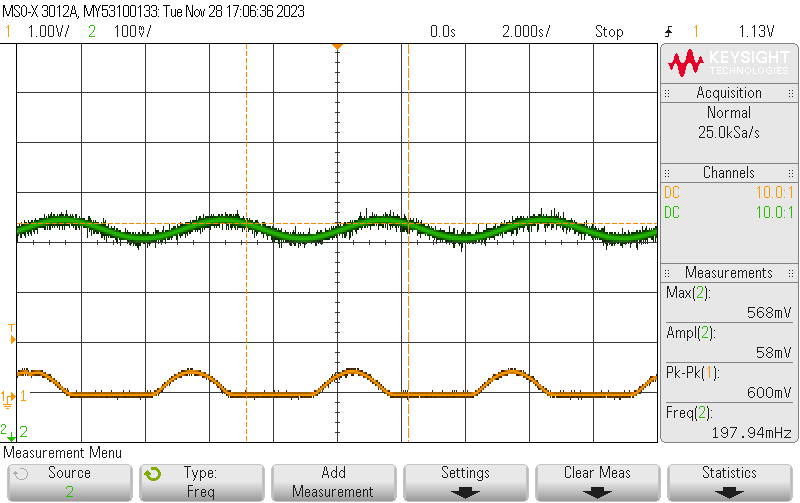
\includegraphics[width=0.75\textwidth]{200mHz.png}
    \caption{Oscilloscope capture at 200 mHz (stop band)}
    \label{fig:200mHzCapture}
\end{figure}

Figure \ref{fig:200mHzCapture} shows that the output of the circuit is a sinusoidal wave with a frequency of 200 mHz, which is the expected behavior. The amplitude of the wave is approximately 0.6 V, which correctly reflects a filtered signal from the OPB745 (in stop band).

Figure \ref{fig:1HzCapture} shows the oscilloscope capture of the output of the circuit at 1 Hz (60 BPM).

\begin{figure}[H]
    \centering
    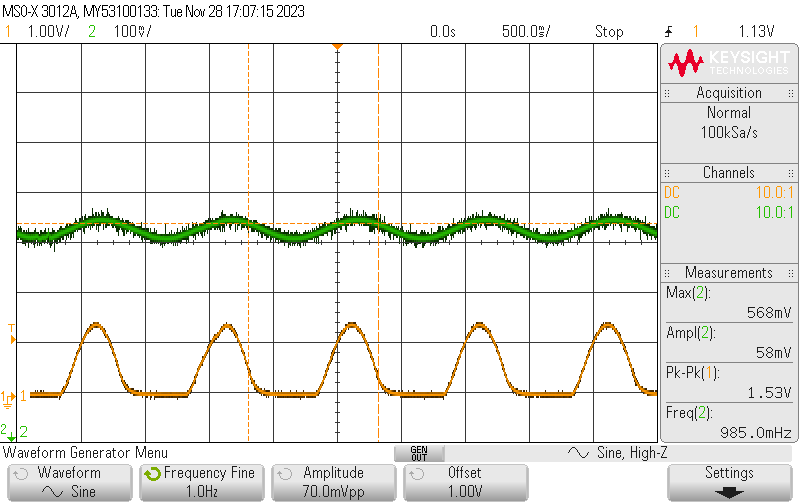
\includegraphics[width=0.75\textwidth]{1Hz.png}
    \caption{Oscilloscope capture at 1 Hz (pass band)}
    \label{fig:1HzCapture}
\end{figure}

Figure \ref{fig:1HzCapture} shows that the output of the circuit is a sinusoidal wave with a frequency of 1 Hz, which is the expected behavior. The amplitude of the wave is approximately 1.53 V, which correctly reflects an amplified signal from the OPB745 (in pass band). The amplitude of the wave is also approximately half of the simulated value, which is attributed to the decreased gain of the high-pass filter of the circuit.

Figure \ref{fig:10HzCapture} shows the oscilloscope capture of the output of the circuit at 10 Hz (600 BPM).

\begin{figure}[H]
    \centering
    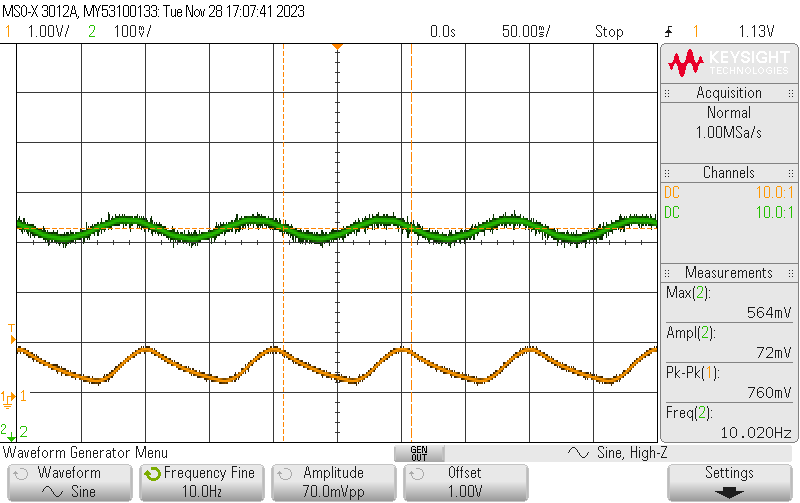
\includegraphics[width=0.75\textwidth]{10Hz.png}
    \caption{Oscilloscope capture at 10 Hz (stop band)}
    \label{fig:10HzCapture}
\end{figure}

Figure \ref{fig:10HzCapture} shows that the output of the circuit is a sinusoidal wave with a frequency of 10 Hz, which is the expected behavior. The amplitude of the wave is approximately 0.76 V, which correctly reflects a filtered signal from the OPB745 (in stop band).

\bigskip

The final output of the circuit was then fed into an MSP432 microcontroller to measure the frequency of the signal. The microcontroller was programmed to measure the frequency of the signal and output the frequency in beats per minute (BPM) to a serial monitor. The microcontroller was programmed to fire interrupts to capture the ADC value of the signal. The ADC value was then converted to a voltage and used to calculate a BPM. The following is the code used:

\begin{verbatim}
#define CAPTURE_FREQ (122)    // frequency of ADC data capture
#define VOLTAGE_CUTOFF (5000) // voltage cutoff for a heartbeat
unsigned int count = 10001;
unsigned int previous = 0;
double prev_bpm = -1;
static char str[100];

// Interrupt Service Routine for Timer32-1
void Timer32_1_ISR(void) {
    char str[30];
    unsigned int num = ADC_In();

    if (num >= VOLTAGE_CUTOFF && previous < VOLTAGE_CUTOFF){
        double bpm = 7320 / count;
        int abs = bpm - prev_bpm;
        if (abs < 0) abs = abs * -1;
        count = 0;
        if (bpm > 40 && bpm < 220 && abs < 11) {
            // print bpm
            sprintf(str, "Heart %d BPM\r\n", (int)bpm);
            uart0_put(str);
        }
        prev_bpm = bpm;
    }
    else { count++; }
    previous = num;
}

int main(void)
{
    DisableInterrupts();
    uart0_init();
    Timer32_1_Init(&Timer32_1_ISR, SystemCoreClock / CAPTURE_FREQ, T32DIV1);
    ADC0_InitSWTriggerCh6();
    EnableInterrupts();
    uart0_put("Initialized\r\n");
    while (1) {}
}
\end{verbatim}

The code shows that the BPM was calculated by counting the number of ADC values that were below a certain voltage cutoff relative to all ADC values. The ADC values were captured at a frequency of 122 Hz. The BPM was then calculated using Equation \ref{eq:bpm}.

\begin{equation}
\text{BPM} = \frac{\text{CAPTURE\_FREQ} \times 60}{\text{count}} \label{eq:bpm}
\end{equation}

The code shows that the BPM was only calculated if the BPM was between 40 and 220 and the difference between the current BPM and the previous BPM was less than 11. This was done to prevent the BPM from fluctuating too much, providing a more stable reading.

The microcontroller was then connected to the circuit and the circuit was tested using a function generator to generate input wave to simulate a heartbeat at different BPM. Figure \ref{fig:serialMonitor} shows the output of the serial monitor.

\begin{figure}[H]
    \centering
    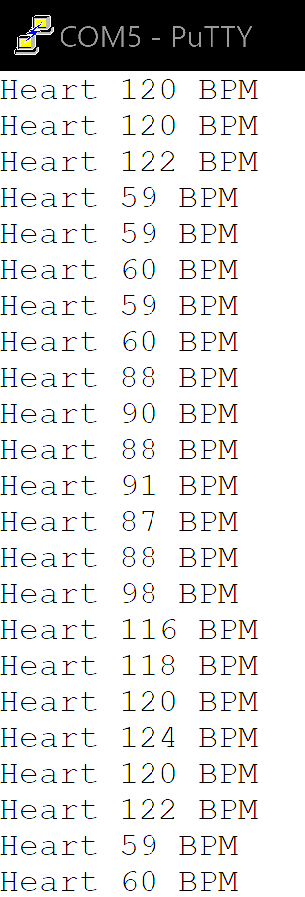
\includegraphics[width=0.2\textwidth]{putty.png}
    \caption{Serial Monitor Output}
    \label{fig:serialMonitor}
\end{figure}

The figure shows that the output of the serial monitor is the BPM of the input wave, which was manually set to 2 Hz, 1 Hz, 2 Hz, and then 1 Hz. The BPM is calculated to to be 120, 60, 120, and 60, respectively, which matches the output shown in the figure. The output also shows slight fluctuations in the BPM of $\pm 1$, which is attributed to noise.

\section*{Questions}

\textbf{1.} \emph{What is the ERC and DRC for?}

ERC stands for Electrical Rule Check and DRC stands for Design Rule Check. The ERC checks for electrical errors in the schematic, such as unconnected pins. The DRC checks for design errors in the schematic, such as incorrect pin types.

\bigskip

\textbf{2.} \emph{Did your circuit cutoff frequencies match your expected/calculated values? Explain}

The cutoff frequency of the low-pass filter of the circuit matched the calculated values. The cutoff frequencies of the high-pass and band-pass filters were slightly different than the calculated values, but were close enough to be considered correct.

\bigskip

\textbf{3.} \emph{Did the gain of the circuit match the expected/calculated values? Explain}

The gain of the circuit was slightly lower than the calculated values, but was close enough to be considered correct, which is attributed to the use of a real op amp instead of an ideal op amp. The gain of the high-pass filter was approximately half of the calculated value, which propagated through the rest of the circuit, causing a decreased gain in the band-pass filter, and thus, the complete circuit.

\section*{Conclusion}

This report details the design, simulation, construction, and testing of a heart rate monitoring circuit. The exercise achieved partial success, demonstrated by the effective performance of the constructed circuit with an oscilloscope-generated sinusoidal signal and its compatibility with the MSP432 microcontroller for heartbeat frequency detection. However, problems and limitations were encountered, such as the inability of the OPB745 sensor in the constructed circuit to detect an actual heartbeat and the gain drop in the high-pass filter stage of the circuit. The experimental results were generally consistent with the simulations, showing slight deviations in cutoff frequencies and gain values, which can be attributed to the practical limitations of real-world components versus idealized simulation models.

\newpage
\begin{figure}[H]
    \centering
    \begin{adjustbox}{center}
        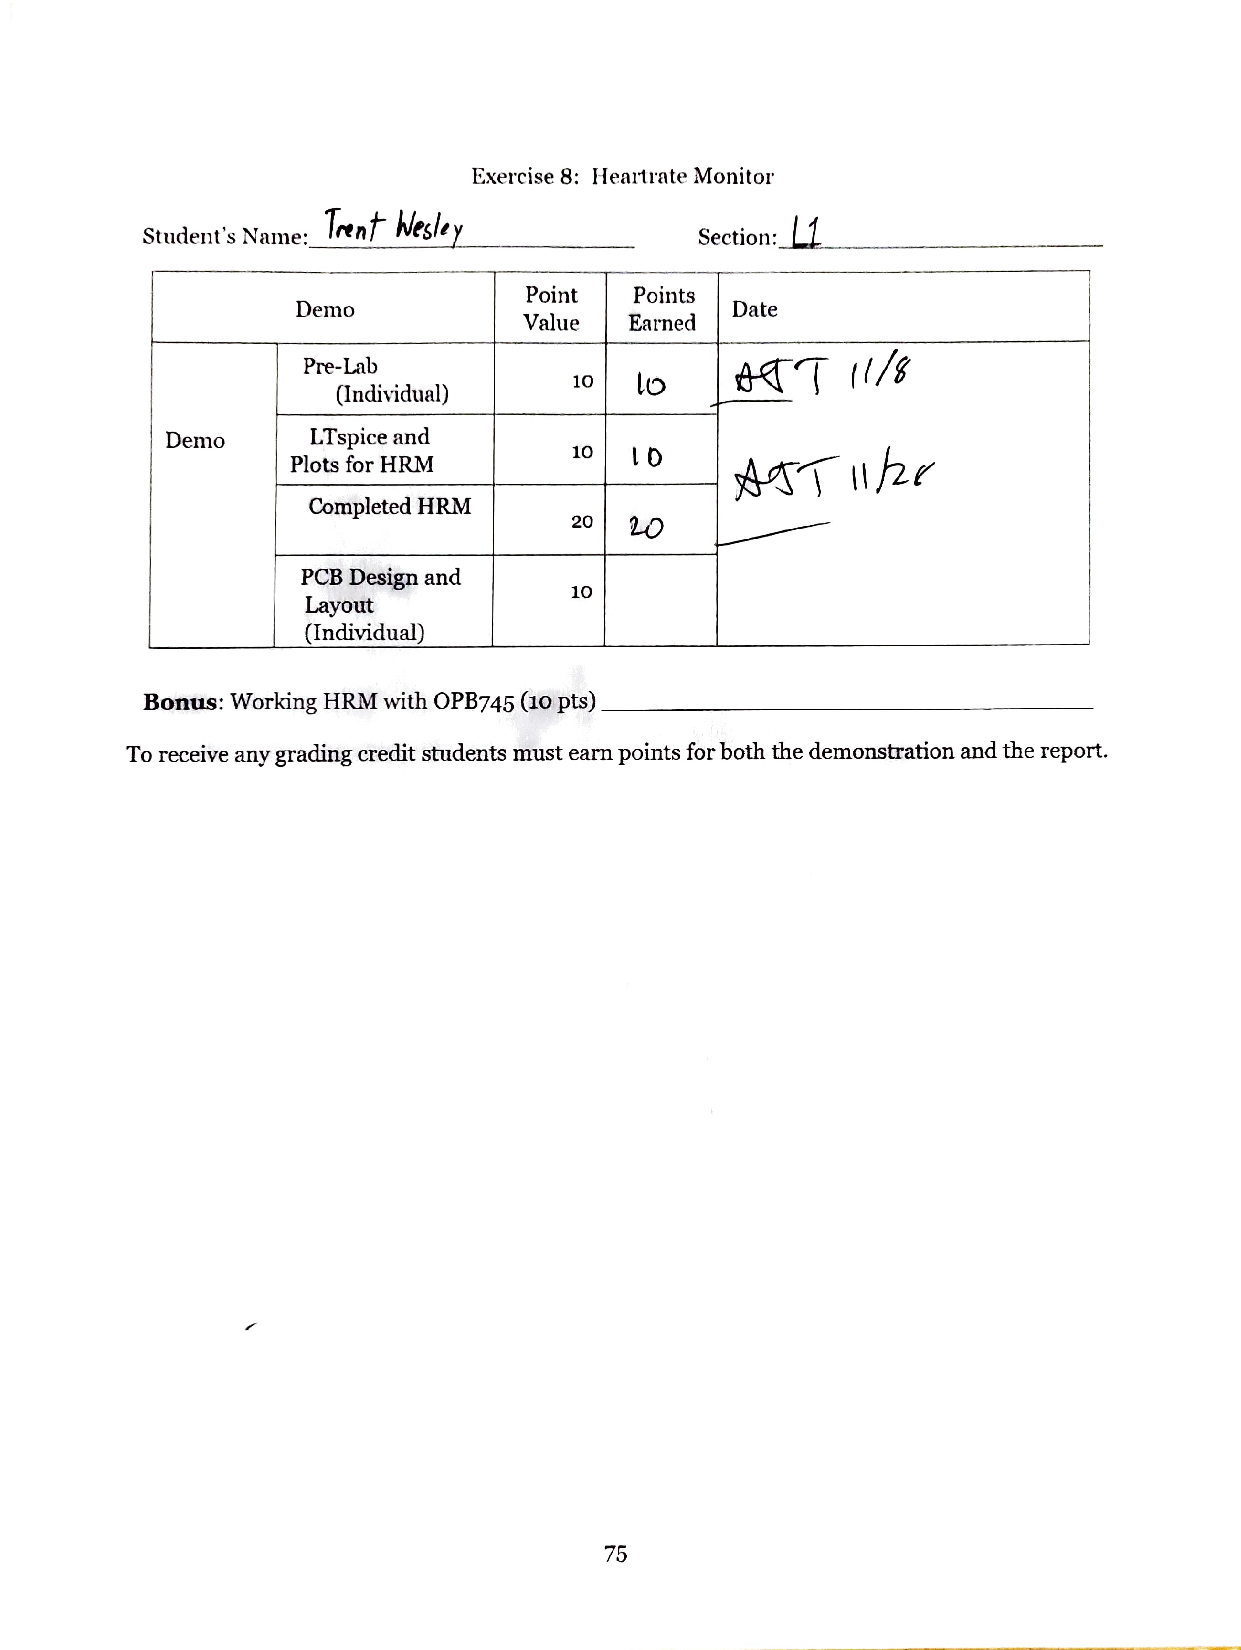
\includegraphics[width=1.26\textwidth]{signoff_1.pdf}
    \end{adjustbox}
\end{figure}

\newpage
\begin{figure}[H]
    \centering
    \begin{adjustbox}{center}
        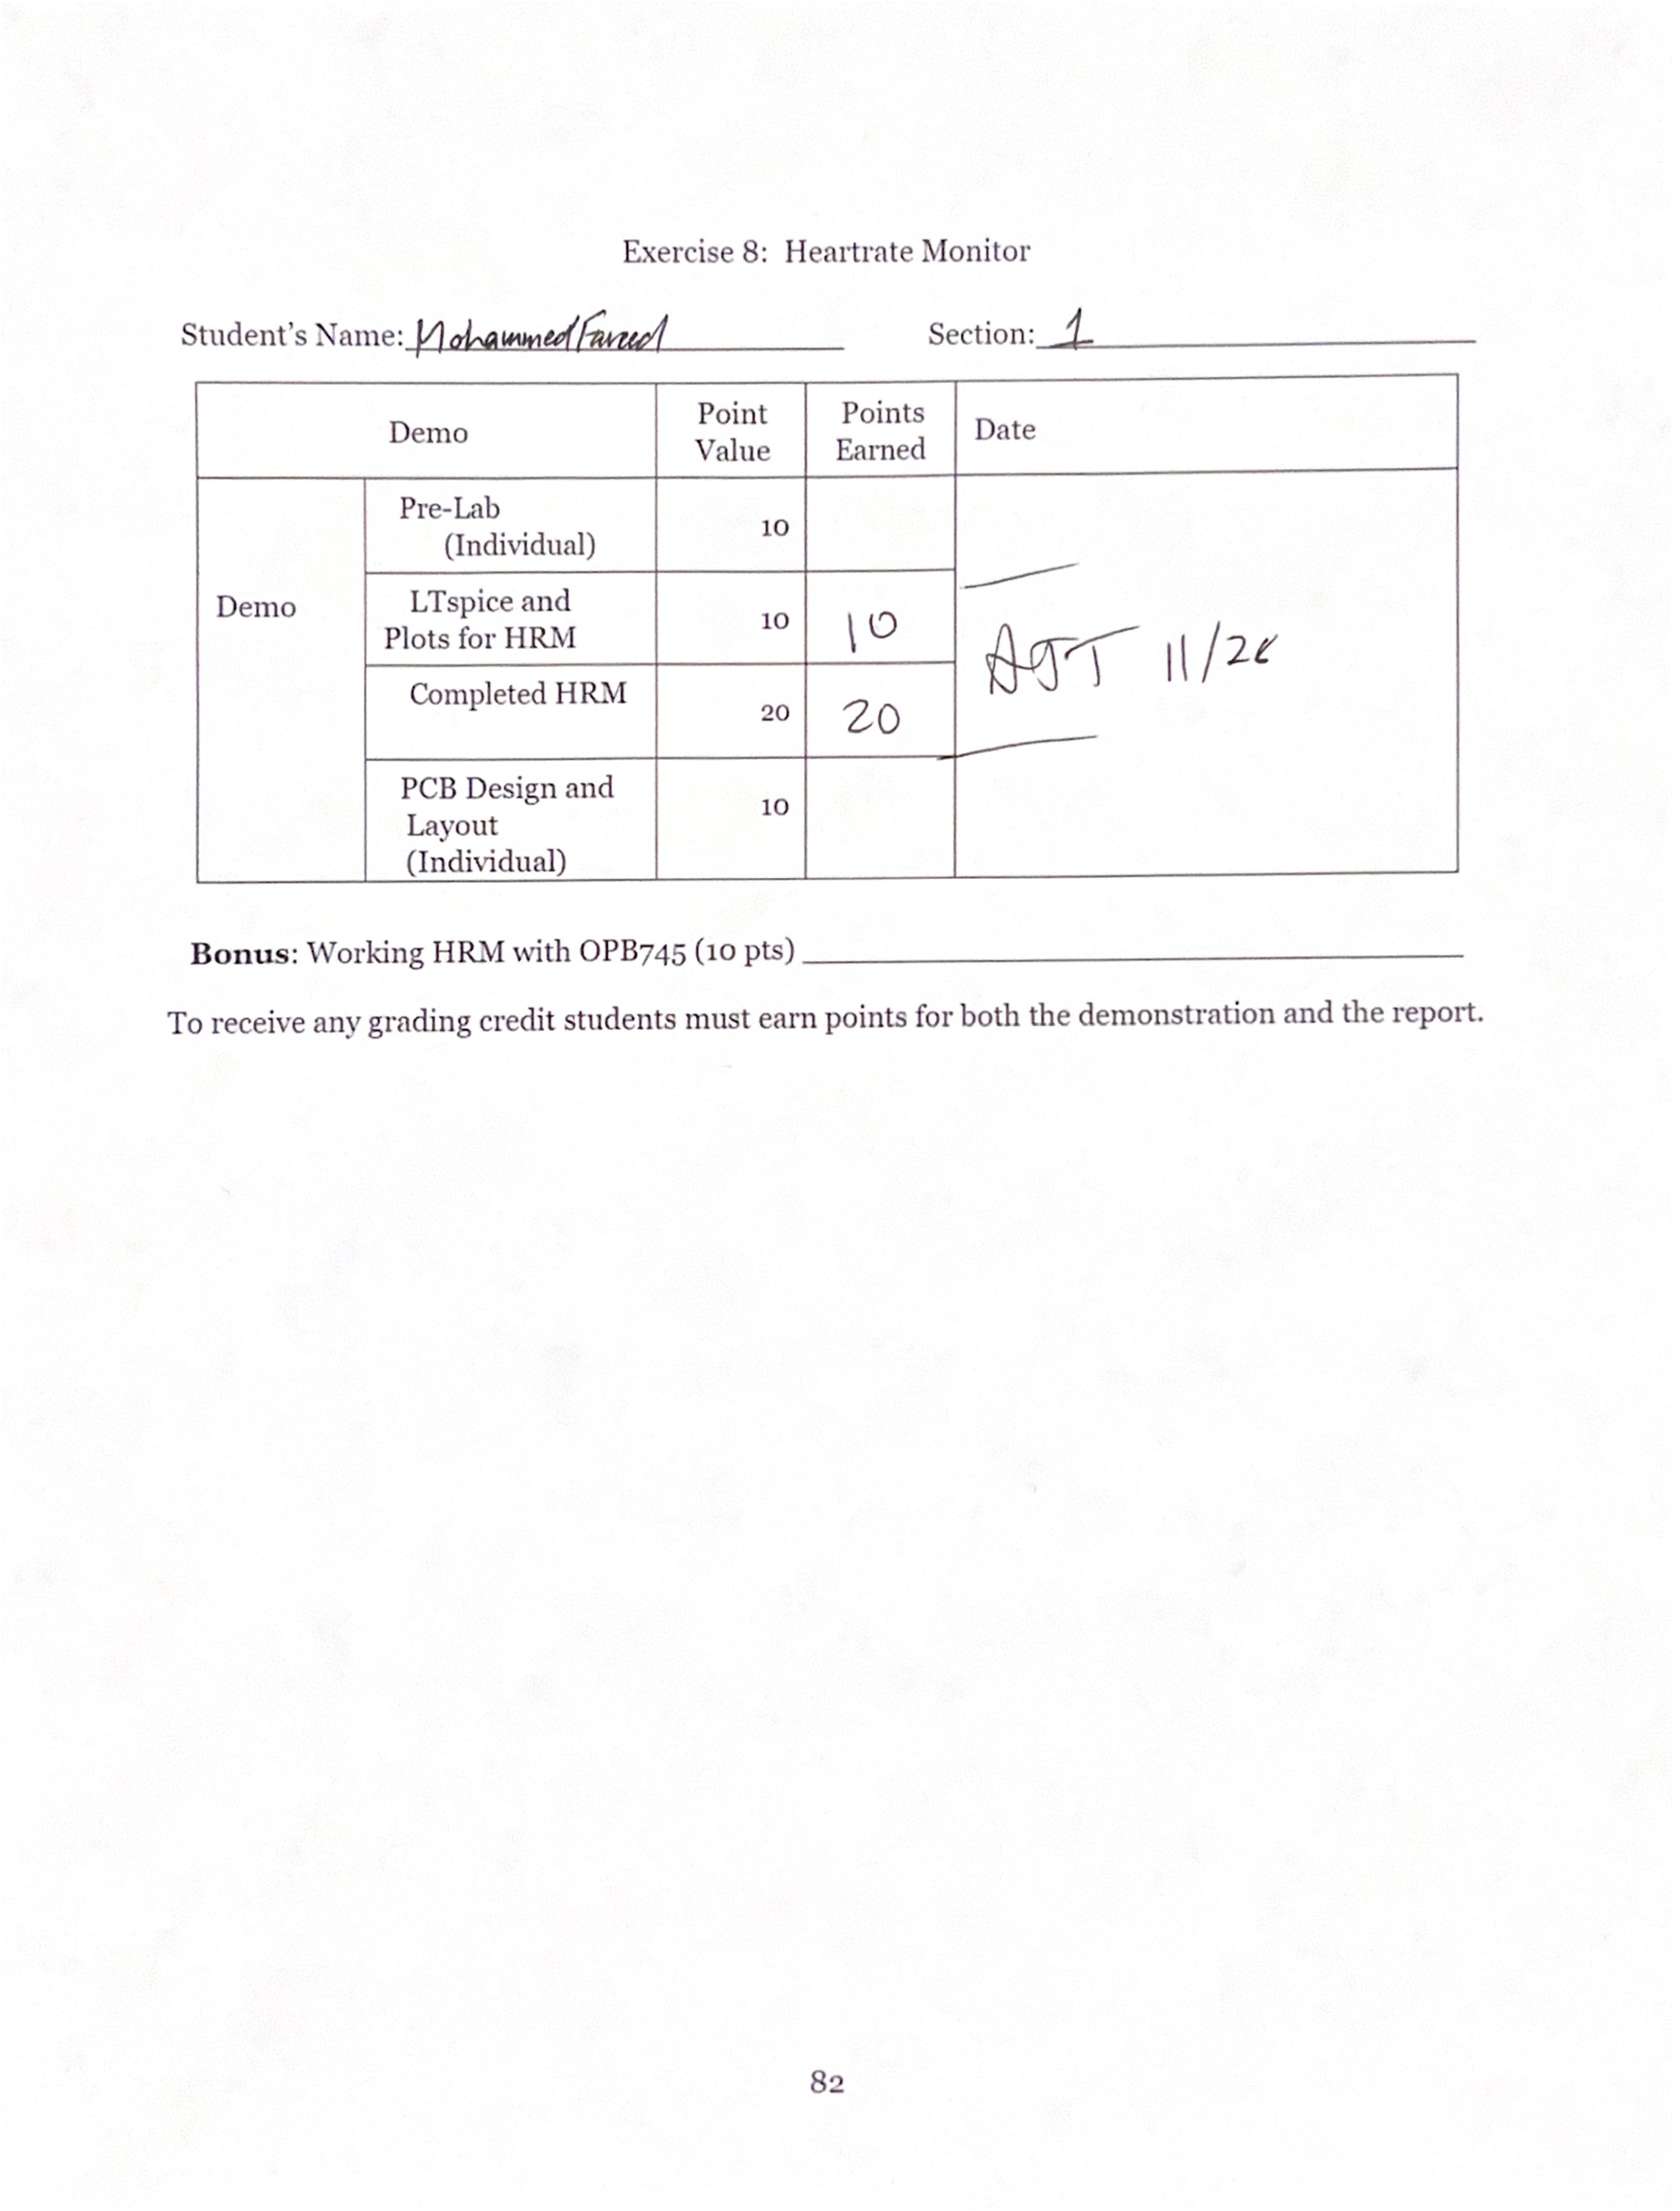
\includegraphics[width=1.26\textwidth]{signoff_2.pdf}
    \end{adjustbox}
\end{figure}

\end{document}
